\documentclass[a4paper]{report}
\usepackage[utf8]{inputenc}
\usepackage{chngcntr}
\usepackage[margin=1in,includeheadfoot,headheight=13.6pt,footskip=2cm]{geometry}
\usepackage{tikz}
\usepackage{amsmath}
\usepackage{pgfplots}
\usepackage{listingsutf8}
\usepackage{graphicx}
\usepackage[main=czech]{babel}
\usepackage[utf8]{inputenc}
\usepackage{graphicx}
\usepackage{amsfonts}
\usepackage[colorlinks=true,urlcolor=blue]{hyperref}
\usepackage{eurosym}
\usepackage{chemfig}
\usepackage[version=4]{mhchem}
\usepackage{multicol}
\usepackage{titlesec}
\usepackage{float}
\usepackage{fancyhdr}
\usepackage{array}
\usepackage{longtable}
\usepackage{dirtytalk}
\pdfminorversion=5 
\pdfcompresslevel=9
\pdfobjcompresslevel=2
\newcolumntype{L}[1]{>{\raggedright\let\newline\\\arraybackslash\hspace{0pt}}m{#1}}
\newcolumntype{C}[1]{>{\centering\let\newline\\\arraybackslash\hspace{0pt}}m{#1}}
\newcolumntype{R}[1]{>{\raggedleft\let\newline\\\arraybackslash\hspace{0pt}}m{#1}}
\newcommand{\comm}[1]{}
\newenvironment{MulticolFigure}
  {\par\medskip\noindent\minipage{\linewidth}}
  {\endminipage\par\medskip}
\title{Závěrečná zpráva Hatalom}
\author{Patrik Novotný, Jakub Suchánek, Lukáš Vőlfl,\\Jan Janoušek, Jakub Zeman, Martin Vítek a vedoucí Mgr. Lenka Vinklerová}
\date{2018}
\counterwithout{section}{chapter}
\newcommand{\sectionbreak}{\clearpage}
\def\tick{\tikz\fill[scale=0.4](0,.35) -- (.25,0) -- (1,.7) -- (.25,.15) -- cycle;}
\pagestyle{fancy}
\fancyhf{}
\fancyhead[RO, LE]{\scshape\nouppercase{\leftmark}}
\fancyfoot[RO, LE]{\thepage}
%\fancyhf{}
\fancyhead[C]{Gymnazium Opatov Space Agency - Hatalom 2018}
\fancyfoot[R]{
\includegraphics[width=30pt]{Logo_final.png}}
\fancyfoot[C]{\thepage}
\renewcommand{\headrulewidth}{0.7pt}
\renewcommand{\footrulewidth}{0.7pt}
\setlength{\parskip}{5pt}
\begin{document}
\begin{titlepage}
    \centering
    \vfil
    
\includegraphics[width=400pt]{Logo_final.png}
    \vfill
    {\bfseries\Large
        Závěrečná zpráva\\
        Hatalom\\
        2018\\
    }
    \vskip2cm
    \large Patrik Novotný, Jakub Suchánek, Lukáš Vőlfl, Jan Janoušek, Jakub Zeman, Martin Vítek\\
    \vfill
    \large Vedoucí Mgr. Lenka Vinklerová\\
    \vfill
    \vfill
\end{titlepage}
% Takto komentujte text.
\comm{nebo takto}
\tableofcontents
\section{Úvod}
\paragraph{} V rukou právě držíte závěrečnou práci shrnující fakta projektu CanSat Hatalom, který stavěli členové GOSA neboli Gymnazium Opatov Space Agency. V posledních šesti měsících jsme založili agenturu GOSA, která zaštítila na našem gymnáziu veškerý vědecký a technický vývoj, nejenom soutěž CanSat. Navázali jsme kontakty, získali peníze, naučili se řádně plánovat, konstruovat a třeba i vymýšlet testy částí projektu, což se ukázalo jako velmi důležité. Také jsme se naučili, jak si dělit práci. Rozhodli jsme se výsledky naší práce poskytnout všem, proto také je náš projekt opensourcovou záležitostí. Projekt byl náročný vzhledem k tomu, že jsme všichni maturanti, ale stál za to a dal nám mnoho. Přečtete-li si tedy další části zprávy, tak nejenže zjistíte, jak co funguje, ale i proč a jak jsme dané řešení zvolili.
\section{Náš tým}
\begin{multicols}{2}
\begin{center}
\begin{MulticolFigure}
\centering
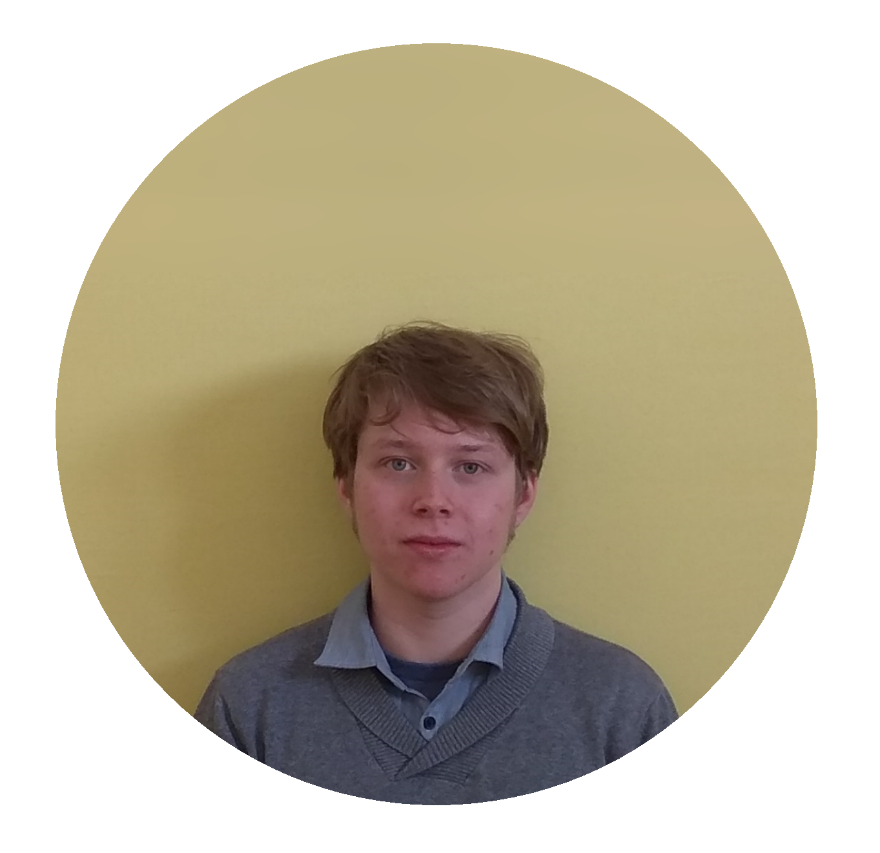
\includegraphics[width=80pt]{patrik.png}
\end{MulticolFigure}
\paragraph{} \large Patrik Novotný – kapitán
\paragraph{} \normalsize Konstrukce desinfekční komory, právo, finance
\begin{MulticolFigure}
\centering
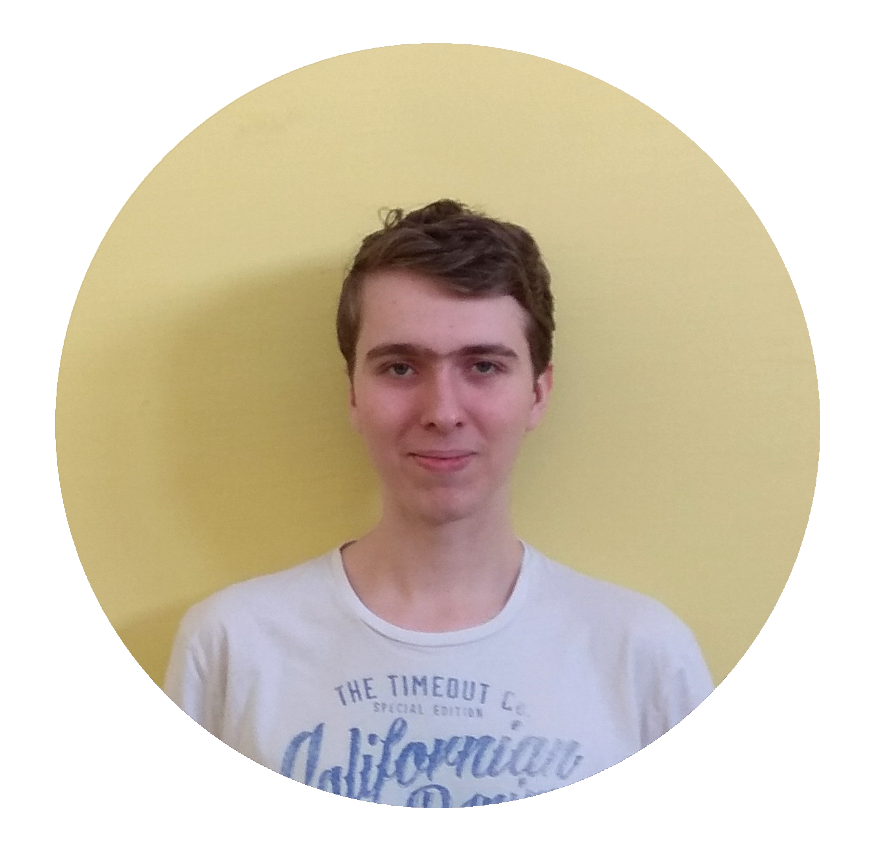
\includegraphics[width=80pt]{suchy.png}
\end{MulticolFigure}
\paragraph{} \large Jakub Suchánek – šéftechnik
\paragraph{} \normalsize Celkový design CanSatu, tvorba softwaru pro řídící obvod
\begin{MulticolFigure}
\centering
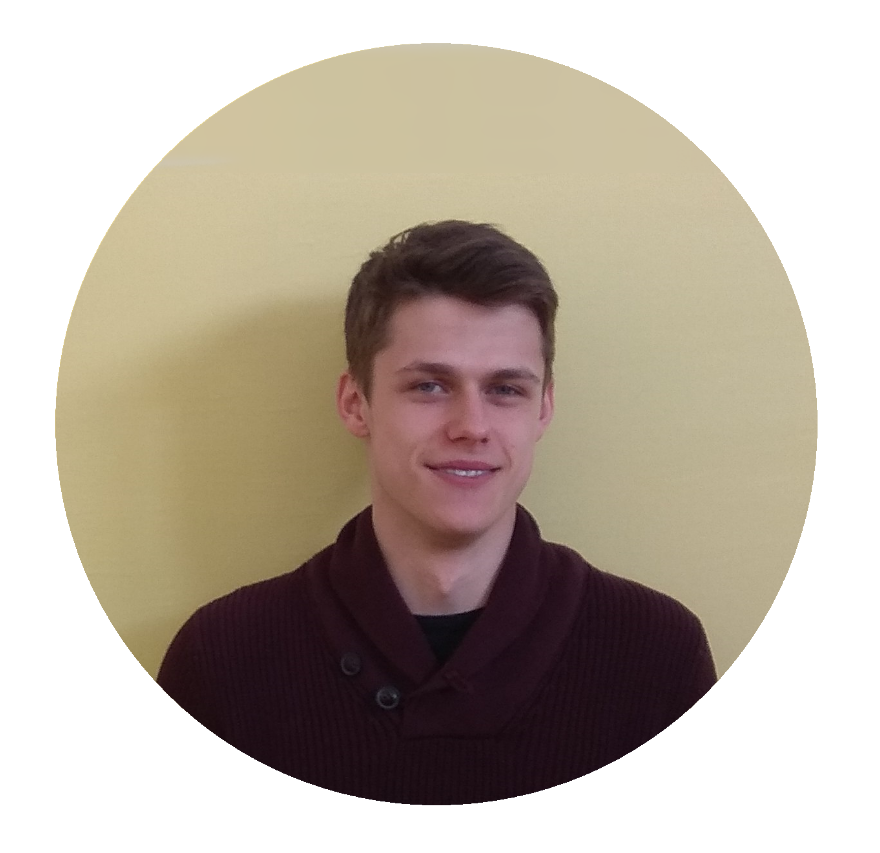
\includegraphics[width=80pt]{lukas.png}
\end{MulticolFigure}
\paragraph{} \large Lukáš Vőlfl – konstruktér, dronař
\paragraph{} \normalsize Ovládání drona při testech, design letových subsystémů
\begin{MulticolFigure}
\centering
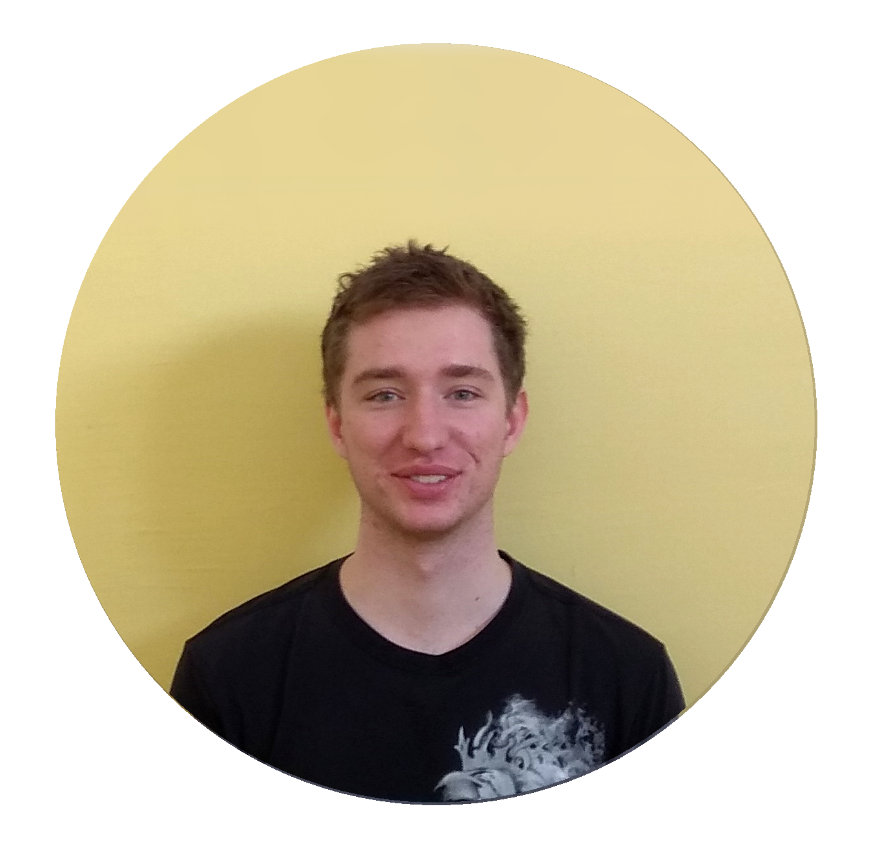
\includegraphics[width=80pt]{honza.png}
\end{MulticolFigure}
\paragraph{} \large Jan Janoušek – PR a HR odborník
\paragraph{} \normalsize Propagace na sociálních sítích, komunikace se sponzory
\begin{MulticolFigure}
\centering

\includegraphics[width=80pt]{zman.png}
\end{MulticolFigure}
\paragraph{} \large Jakub Zeman – konstruktér, bezpečnost práce
\paragraph{} \normalsize Pájení, sestavení a opravy CanSatu
\begin{MulticolFigure}
\centering
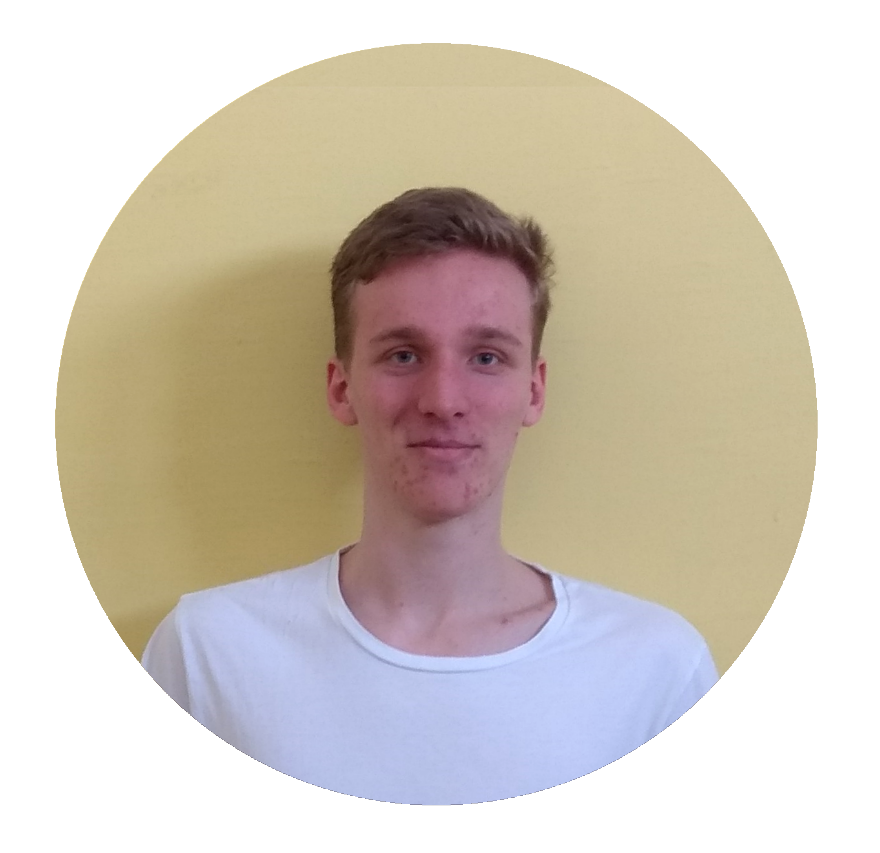
\includegraphics[width=80pt]{vitek.png}
\end{MulticolFigure}
\paragraph{} \large Martin Vítek – programátor
\paragraph{} \normalsize Vývoj webu, finance
\end{center}
\end{multicols}
\paragraph{} Mimo svoje pozice se dělíme do týmů dle daného úkolu - hlavně programátorský (Jakub Suchánek, Patrik Novotný a Martin Vítek) a konstrukční (Jakub Zeman, Lukáš Vőlfl a Jakub Suchánek), Jan Janoušek obstarává provozní činnosti.
\subsection{Letové pozice}
\paragraph{} Speciálně pak máme vyčleněny pozice pro let (v současné době se prakticky týká pouze testů komponent). Pro neexistenci českých ekvivalentů užíváme anglických názvů:
\paragraph{} Mission Manager – Patrik Novotný
\paragraph{} Payload Manager – Jakub Suchánek
\paragraph{} Flight Director – Lukáš Vőlfl
\paragraph{} Safety Officer– Jakub Zeman
\section{Průběh prací}
\begin{itemize}
\item Říjen: Na začátku října jsme začali rozmýšlet, jakou si zvolíme sekundární misi. Měli jsme tři různé varianty řešení a to:
\begin{itemize}
\item Řiditelný padák
\item Letadlo
\item Dron/Helikoptéra
\end{itemize}
Každý si vybral, která z variant se mu líbí, a snažil se ji obhájit a zároveň oponovat volbám ostatních. Tímto postupem jsme dospěli k závěru, že nejvhodnější a nejzajímavější řešení bude dron.
\item Listopad: Po definitivním rozhodnutí, že náš CanSat bude fungovat na způsob dronu, jsme začali kreslit návrhy a hledat optimální řešení konstrukčních problémů, např. způsob vysouvání ramen s rotory. Zároveň Jakub Zeman (po dlouhém rozvažování, zda anténu koupit nebo postavit) za pomoci různých všedních i nevšedních nástrojů (lahev od kečupu) vyrobil anténu. Dne 9. listopadu jsme se sešli s Klubem přátel gymnázia Opatov (KPGO) a požádáli o sponzoring. Náš projekt se jim velice líbil a slíbili nám finanční podporu.
\item Prosinec: Jakub Suchánek začal rozkreslovat základní desku. Řešíme co všechno budeme chtít měřit a jaké senzory na CanSat dáme. V tomto rozhodování nám pomohla schůzka s Janem Horákem, který je členem týmu RAJsat, jenž v soutěži zvítězil v letech 2016 a 2017. Ukázal nám poslední verzi jejich satelitu, s nímž se zúčastnili evropského finále v roce 2017. I přesto, že jejich satelit se od naší vize výrazně lišil, odnesli jsme si ze setkání spoustu informací a inspirace. Honza nám dal spoustu rad vycházejících z jeho zkušeností, neboť nám i v následujících měsících poskytoval konzultace.
\item Leden: V lednu nás čekalo národní semifinále a tudíž byl nejvyšší čas testovat měření a přenos základních dat. Hned 4. ledna jsme se sešli za účelem otestovat spojení a kvalitu antény. Bohužel se vyskytla chyba, kterou se nepodařilo na místě opravit, takže jsme nedokázali vysílat ani na dva metry. Po prvním neúspěchu jsme se znovu sešli o týden později. Plán byl otestovat anténu na vzdálenost 1 km. Po úspěchu se skupinka s přijímací anténou rozhodla přesunout dále. Po dalším úspěchu jsme šli ještě dál. Nakonec jsme bez jakýchkoliv problémů jsme vysílali z Pankráce na Háje, což odpovídá vzdálenosti zhruba 6,5 km. Dále jsme nepokračovali, bylo to zbytečné a těžko by se hledalo místo, ze kterého by bylo možné přímé spojení.
\item Semifinále: 30. ledna nás čekalo republikové semifinále. Setkali jsme se v 8:30 na Opatově a přesunuli se před kancelář ESERO, kde jsme ještě trénovali prezentaci a ladili poslední detaily. První částí semifinále byl telemetrický test, kterého jsme se nijak nebáli, protože naše předchozí testy potvrdily kvalitu spojení. Druhou částí byla prezentace, ve které každý zmínil to hlavní, čím se zabýval, a společně jsme předložili naši vizi CanSatu s plány do budoucna. Porotě se náš nápad líbil, avšak  upozornila nás na jeho složitost a absenci příběhu, ten potom Patrik Novotný vytvořil a je k nalezení na našich webových stánkách a níže v této zprávě. Po odprezentování jsme odešli s pocitem dobře odvedené práce. Odpoledne byly zveřejněny výsledky a my jsme byli šťastni z třetího místa a z postupu do finále. Byla to odměna za naši dosavadní práci, ale i velký závazek do budoucna.
\item Únor: Po uspěšném postupu do národního finále, byl čas začít nakupovat potřebné díly. Zároveň jsme probírali možná řešení problémů jako sebrání vzorku půdy nebo přenos dat na web. V půlce února přišly součástky na pájení hlavního plošného spoje, a tak se Jakub Suchánek pustil do pájení, které bylo možné sledovat live na YouTube. Dne 22.února jsme se sešli u Lukáše Vőlfla za účelem testů stabilizačního padáčku a vypouštěcího zařízení. Porovnáním letu/pádu s padáčkem a bez něj jsme mohli brát testy za vydařené. Nejen, že padáček plechovku stabilizoval do správné polohy, ale i pád výrazně zpomalil. Honza Janoušek zajišťoval logistické úkoly.
\item Březen: Začátek března se nesl v duchu biologie. Patrik Novotný zkoušel, za jak dlouho vyroste na agaru kolonie bakterií z hlíny a pak i ze země. Také vyrobil UVtrubku (níže specifikována).  V půlce měsíce Jakub Zeman začal tisknout testovací CanSat hull, tudíž jsme se mohli připravovat na letové zkoušky. Dne 29. března jsme měsíc zakončili prvním testovacím letem Kosta Moisid, pojmenovaném po podporovateli. Během daného dne tým Jakub Zeman a Jakub Suchánek vyzvedl v Liberci finální a záložní verzi CanSatu. Součastně druhý tým v Praze testoval první let za pomocí motorů. Test dopadl úspěšně a potvrdilo se, že náš koncept je plně funkční a stačí ho do finále optimalizovat.
\item Duben: Měsíc jsme začali workshopem hned 1. dubna, kdy jsme testovali generátor \ce{O3}, zároveň jsme programovali a začali s přípravou průběhové zprávy. Celý duben do finále jsme testovali hardware i software a psali závěrečnou zprávu, v čemž nám pomáhaly konzultace s RajSat týmem. Největší událostí měsíce bylo jednání 9. dubna s KPGO, jelikož nás tento subjekt právně i finančně zajišťuje. Vysvětlili jsme průběh činností a výhledy do budoucna. KPGO schválilo, že při absenci další sponzorů, nám plně uhradí cestu na případné evropské kolo. Následně jsme si otevřeli ve škole stánek a prezentovali dosavadní vývoj projektu zletilým studentům, rodičům a podporovatelům naší školy. Zlatým hřebem měsíce pro nás bude CanSat národní finále na letišti Letkov a v Plzni 19. a 20. dubna. 
\end{itemize}
\section{Testy}
V průběhu projektu jsme podrobili jednotlivé součásti i celý CanSat sérii testů, ty nejdůležitější zde uvádíme.
\paragraph{} Testy padáčku proběhly během výběru variant, což bylo v průběhu listopadu. Ověřili jsme si stabilizační roli padáčku.
\paragraph{} Telekomunikační test 1 - bohužel neúspěšně jsme v průběhu ledna testovali přenos telemetrických dat.
\paragraph{} Telekomunikační test 2 - o týden později jsme provedli test znovu. Povedlo se nám přenášet data každou vteřinu na vzdálenost 6,5 kilometru v rozsahu směrování přijímací antény 20 stupňů.
\paragraph{} Crashtest a test padáku - v lednu jsme testovali výsledný padák a jeho schopnost otevřít ramena CanSatu a přibržďovat. Zde byl stále modelem rýžový CanSat, testy skončily crash testem, který nám sdělil, jak pevný musí být výsledný hull.
\paragraph{} UV testy probíhaly v březnu, kdy jsme nejprve testovali růst bakterií ze vzorku (hlína) i ze vzduchu a učili se poznat, jak daný organismus roste s časem. Následně jsme tyto organismy a květinu osení ozařovali UVC zářivkou.
\begin{figure}[H]
\caption{Biologické pokusy, zdroj: Patrik Novotný}
\centering
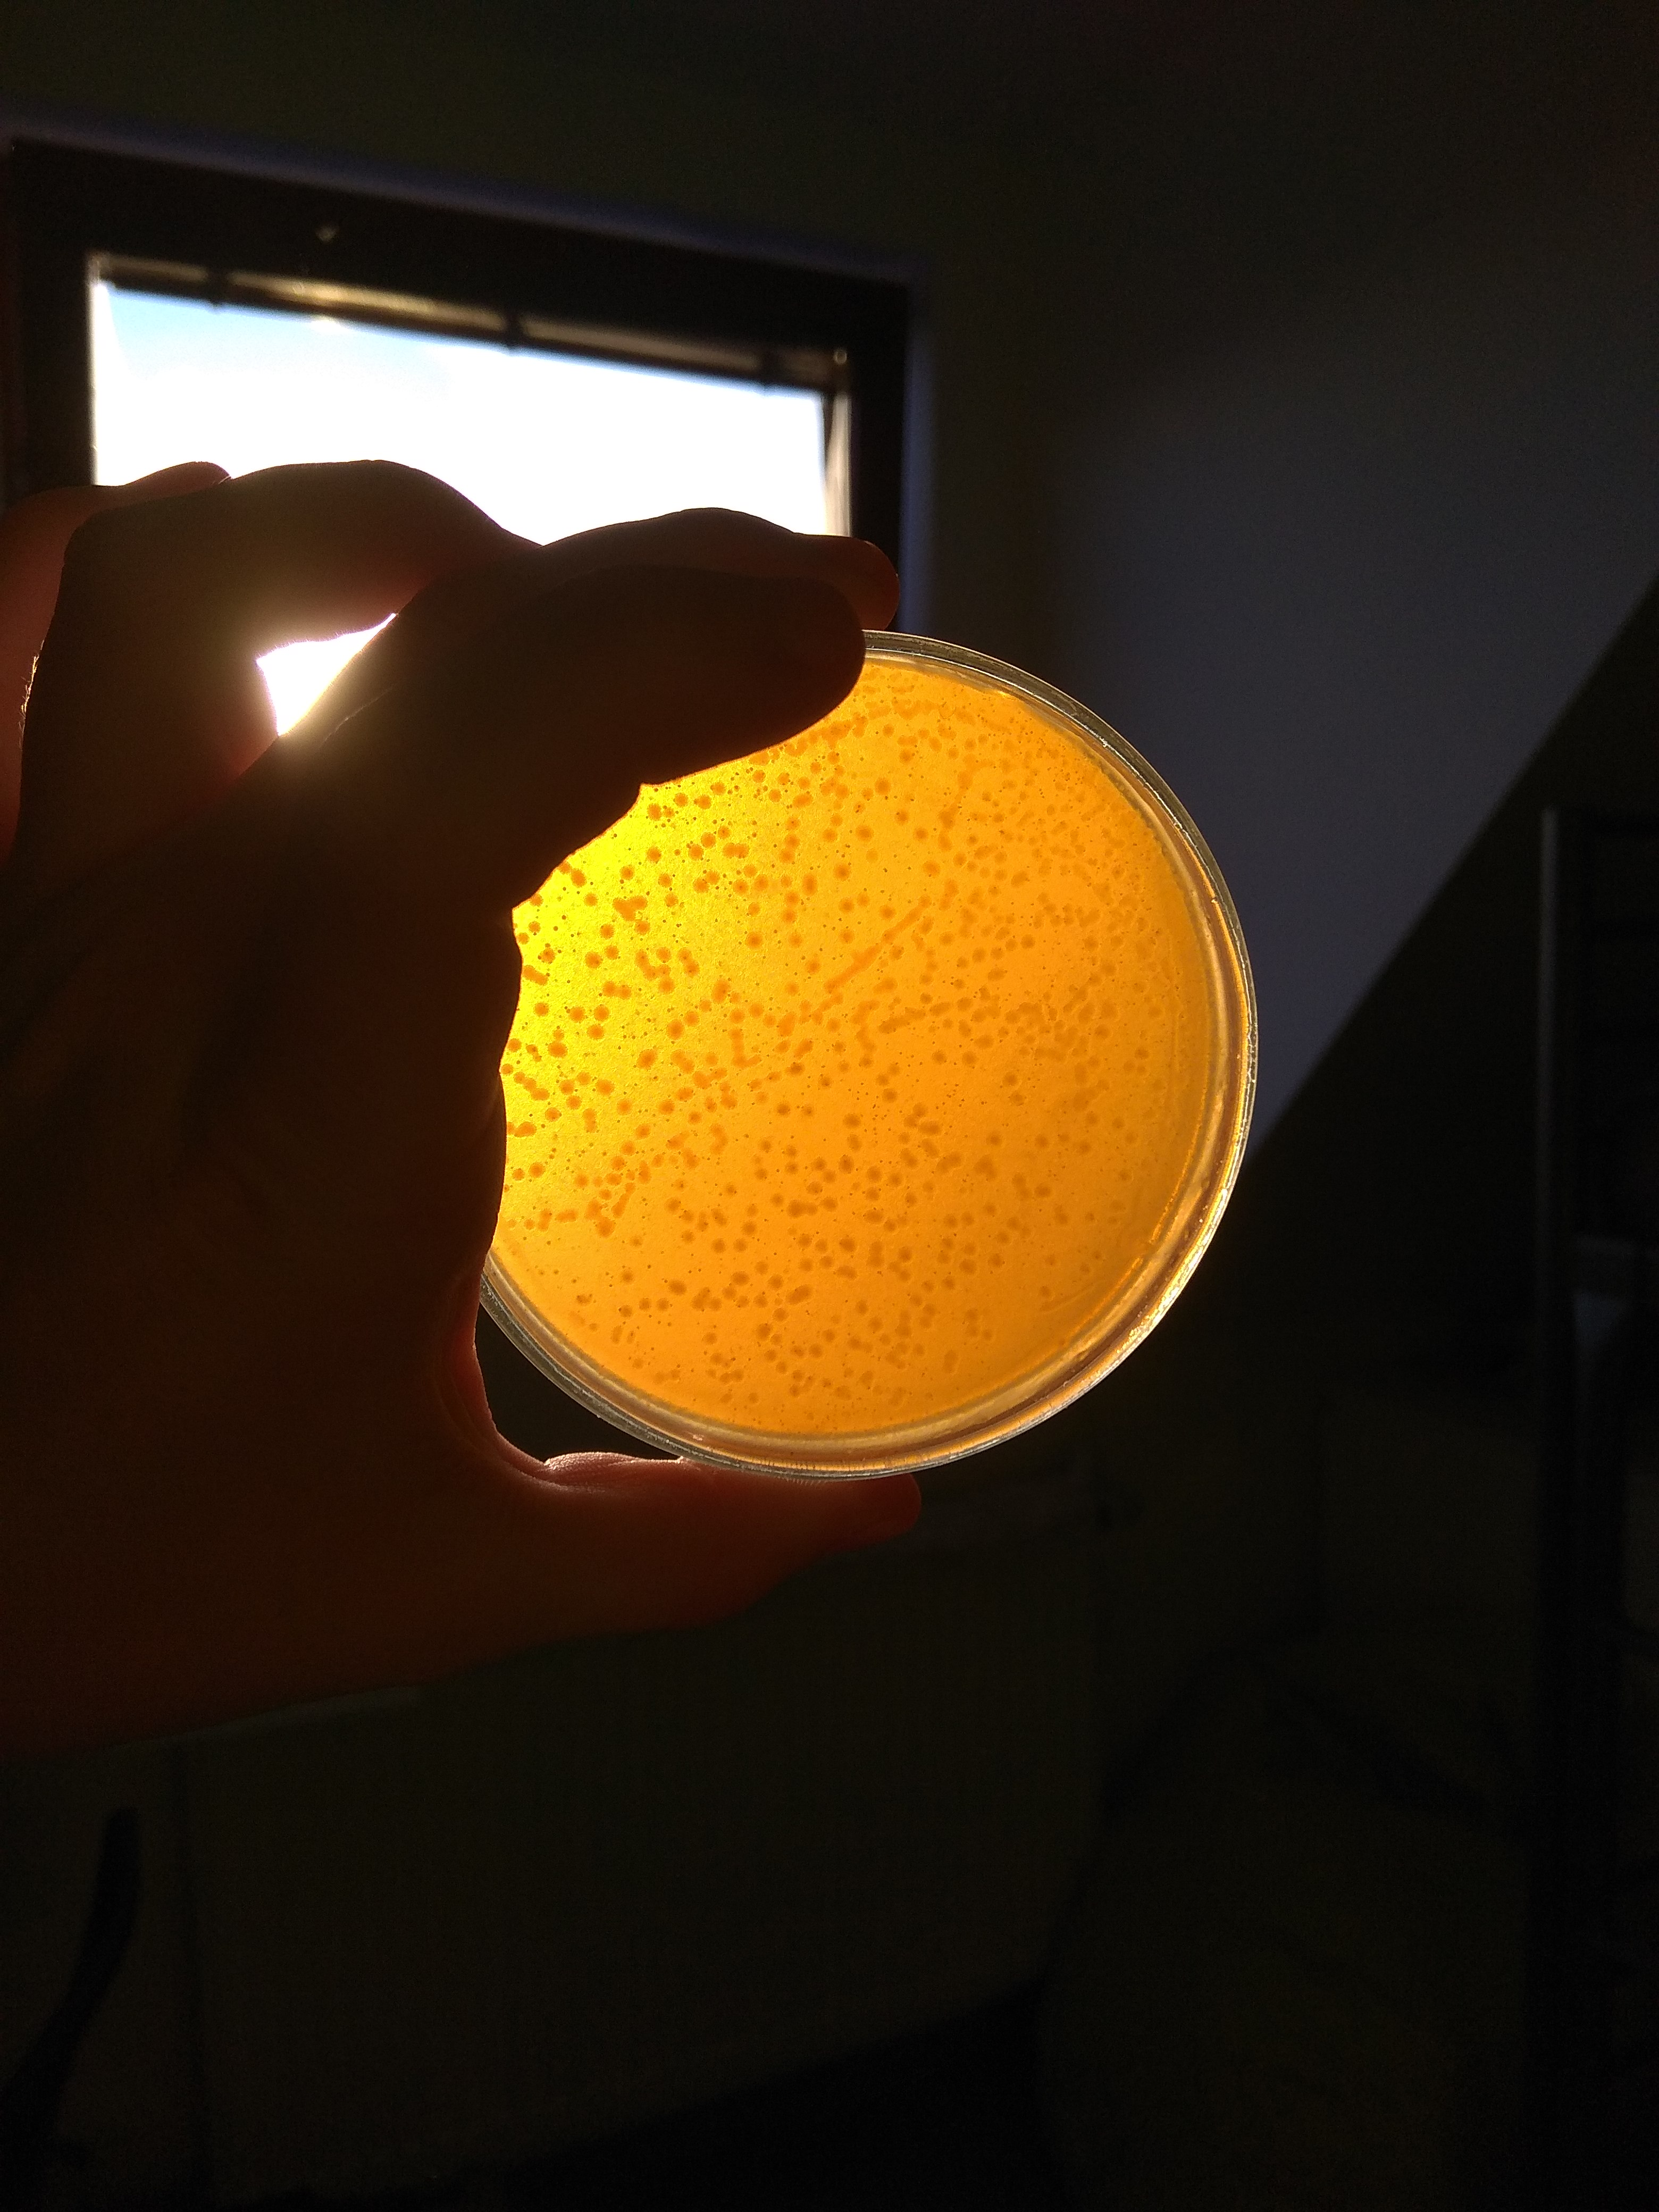
\includegraphics[width=400pt]{Biopokusy.jpg}
\end{figure}
\paragraph{} Test Kosta Moisidis - První kompletní test, kde CanSat letěl v celku. Byl však pro jistotu ovládán dálkově. Test dopadl velmi úspěšně.
\paragraph{} Test Pepa Vu - Zde jsme testovali schopnost chytit CanSat do naší plachty o ploše 48 čtverečních metrů. Po počátečních nezdarech jsme se této nouzové činnosti naučili.
\paragraph{} Test všech systémů - finální test všech systémů nás čeká 15. dubna, kdy chceme testovat CanSat podmínkami tvrdšími, než čekáme.
\section{Příběh}
\paragraph{} Za každou událostí v dějinách stojí příběh, protože právě příběhy jsou tím, co člověka motivuje k činnosti. Jaký je náš příběh? Proč stavíme meziplanetární sondu? Simulujeme misi, ke které možná jednoho dne dojde. Cílem našeho zájmu je planeta obíhající kolem jiné hvězdy, která se jmenuje Kepler 62, okem byste ji neviděli. Je menší než Slunce. Z našich zemí se zdá, že nám obíhá vysoko nad hlavami v souhvězdí Lyry. Je od nás vzdálena skoro 1200 světelných let.
\begin{figure}[!h]
\centering
\caption{Soustava Kepler 62, zdroj:
\href{https://www.nasa.gov/mission_pages/kepler/multimedia/images/kepler-69-diagram.html}{NASA Ames/JPL-Caltech}}
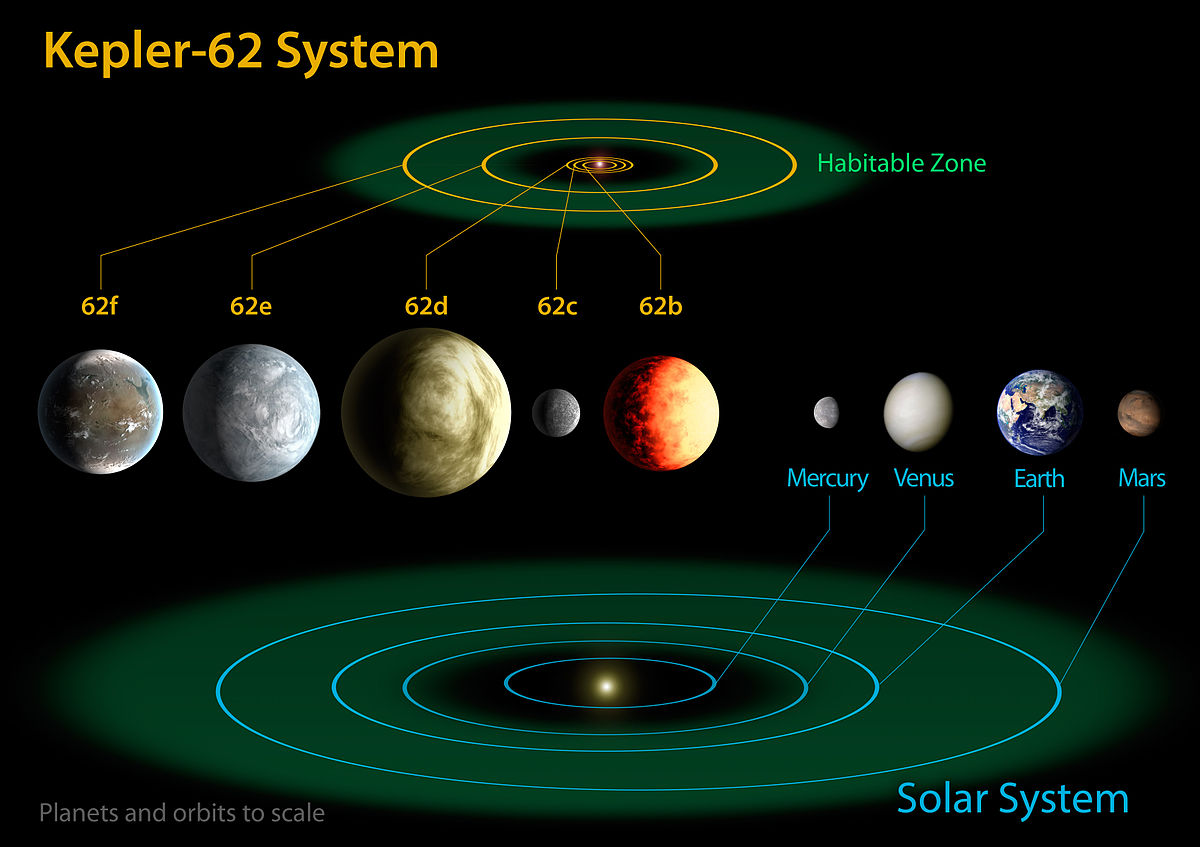
\includegraphics[width=400pt]{Kepler62.jpg}
\end{figure}
\paragraph{} Hvězd je ve vesmíru mnoho, astronomové by vám řekli, že v každé galaxii jich je přibližně \(10^{12}\) a tolik je i ve vesmíru galaxií. O to ale nejde. Je jich mnoho. A některé z nich mají i své planety. Kepler je právě takovou hvězdou, obíhá ho dle našich poznatků 5 planet, dvě obzvlášť zajímavé, označované jako „e“ a „f“. 
\paragraph{} Planeta „e“ leží na vnitřním okraji obyvatelné zóny. Jednoduše řečeno, předpokládáme-li podmínky pro vznik života, pak je moc teplá, má podobnou smůlu jako naše Venuše. Ovšem její sourozenec Kepler 62 f je nadějnější. Nemáme zdaleka všechna data, ale víme, že v dané oběžné vzdálenosti by planeta měla mít průměrnou povrchovou teplotu kolem -40 stupňů. Ovšem pokud by měla tlustší atmosféru (pětkrát) tvořenou \ce{CO2}, což není nic neobvyklého, pak by na většině povrchu planety mohla existovat voda v kapalném skupenství. Při tenčí atmosféře by se voda v kapalné fázi mohla vyskytovat jen v některých částech planety.
\paragraph{} Nyní ovšem k optimističtějším datům. Hvězda Kepler 62 je stabilní hvězdou (nízká hmotnost i metalicita vůči Slunci), navíc by měla zářit ještě dvakrát déle, než je stáří vesmíru. Planeta oběhne svou domovskou hvězdu za 267 dní, hvězda by ji tudíž neměla příliš negativně ovlivňovat. Celý systém je dle odhadů až o dvě miliardy let starší než náš. Naše cílová planeta má také pravděpodobně vlastní měsíc a skloněnou rotační osu, takže se na jejím povrchu mění roční období. Z těchto údajů lze odhadnout, že není lepší kandidát pro nalezení mimozemského života, byť lze předpokládat nižší stupeň vyspělosti vzhledem k tomu, že z planety nepřijímáme vysílání.
\paragraph{} Co a proč tedy hodláme na planetě uskutečnit?
\begin{itemize}
\item Z orbity získáme snímky planety – v našem případě Google Maps, dle snímků vybereme místo přistání.
\item Po průletu atmosférou rušící vysílání zahájíme samotnou misi – příjem signálu bude možný z výšky kolem 1-2 km nad povrchem, budeme udržovat rychlost klesání 6-12 m/s, abychom nepoškodili aparaturu v sondě ani nenarušili přenosy dat uskutečňované více způsoby.
\item Celou dobu letu budeme vysílat obraz. Je možné, že sice již nežije na planetě vyspělá civilizace, ale třeba žila a její pozůstatky budou viditelné.
\item Budeme měřit údaje nutné pro vznik života – množství \ce{CO2} a \ce{O2}, tlak a teplotu, a dále intenzitu magnetického pole
V poslední fázi mise odebereme malý vzorek horniny a zjistíme, zda nám v agaru nevyroste bakteriální život blízký pozemskému.
\end{itemize}
\paragraph{} Na reálnou misi na Kepler 62 f si budeme muset jistě nějakou dobu počkat, ač se dá očekávat, že to bude jeden z prvních lidských mezihvězdných cílů. Na simulaci mise však čekat nemusíme!
\section{Plánovaný průběh mise}
\subsection{Předletová příprava}
\paragraph{} Před startem CanSatu je nutno zkontrolovat a popř. dobít baterie CanSatu. Poté vyberou pořadatelé místo dopadu z mapy, to se zanese do Groundstation. Zapne se a zkalibruje jak GPS, tak flight controller, který musí být zapnut v rovnovážné poloze. Mezi tím bude v UV trubce ozařována mistička s agarem a rypadlo CanSatu. Při tomto ozařování vzniká \ce{O3}. Poté, co se UV trubka vypne, tak se do ní vloží pro větší dekontaminaci celý CanSat, v němž \ce{O3} zahubí další bakterie, avšak narozdíl od UV záření nepoškodí jeho vnitřní vybavení. Následně může CanSat Hatalom odstartovat. Tento způsob dekontaminace jsme otestovali na mikroorganismech i rostlinách, na zvířatech jsme tak z etických důvodů nečinili.
\subsection{Průběh letu}
\paragraph{} Po vypuštění satelitu se otevře malý padáček sloužící jak ke stabilizaci, tak k mírnému brždění. Vlivem uvolnění CanSatu dojde k otevření ramen a spuštění motorů. CanSat bude automaticky pomalu klesat k místu, které před startem zvolili pořadatelé jako místo přistání. Polohu si v průběhu letu CanSat kontroluje pomocí tlakoměru a GPS. Když se přiblíží k zemi na vzdálenost metrů, tak začne vyhodnocovat vhodné místo k přistání. Pomocí čidel vzdálenosti najde místo podobně vzdálené od všech čtyř čidel (bude se tedy jednat o rovinu) a pak přistane. Po přistání rýpne lopatka na servomotorku do země a následně do agaru, v něm po kontaktu s hlínou začne bujet život. Po celou dobu letu i po přistání bude CanSat odesílat údaje o teplotě, tlaku, poloze a množství \ce{CO2}.
\subsection{Vyhodnocení dat}
\paragraph{} Všechna naměřená data se budou posílat do Groundstation a odtud poputují na webové úložiště na našich stránkách. Už během letu se bude na webovkách objevovat poloha CanSatu v reálném čase. Ostatní data se budou zobrazovat na webu, ale vyhodnocovat a dávat do souvislostí se budou až po letu. Po vyjmutí misky s agarem ji Patrik Novotný nafotí a následně prozkoumá mikroskopem, analýzu zkoušel již doma. Stopy života je schopen analyzovat. S další analýzou (s co nejpřesnější identifikací - skupiny organismů či dokonce samotného druhu) mu pomůže po Skypu s námi spolupracující biologická konzultantka Barbora Haláková.

\section{Hardwarové vybavení CanSatu}
\begin{figure}[H]
\caption{Schéma plošného spoje, zdroj: Jakub Suchánek}
\centering
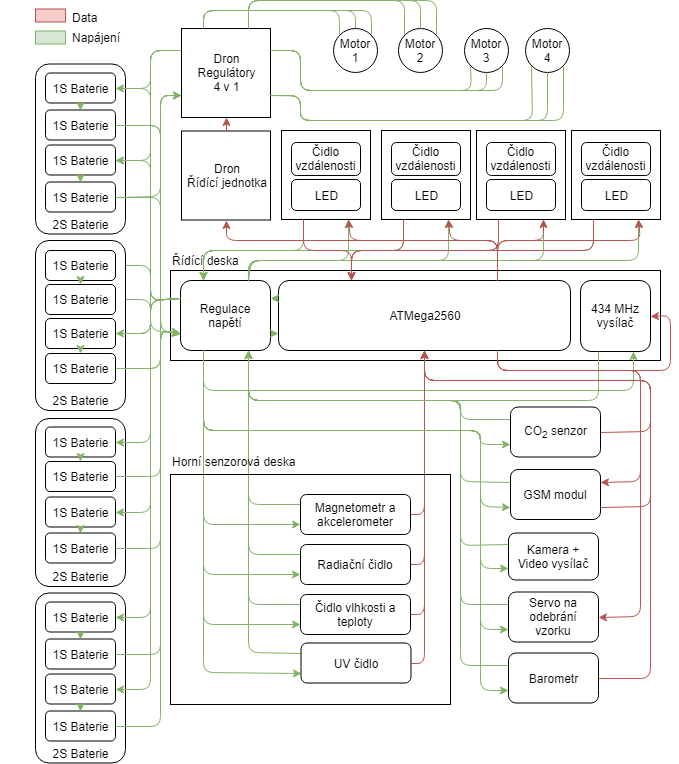
\includegraphics[width=400pt]{CanSat_cz.png}
\end{figure}
\subsection{Řídící deska}
\paragraph{} Deska postavená kolem mikrokontrolleru ATmega2560-16AU, abychom mohli použít software pro Arduino Mega 2560 a knihovny pro komunikaci Arduina a ostatních elektronických součástek. Obsahuje regulaci napětí, napěťové převodníky na signálních cestách, konektory pro všechny ostatní desky a komponenty a modul pro rádiové vysílání.
\begin{figure}[H]
\centering
\caption{Řídící deska shora, zdroj: Jakub Suchánek}
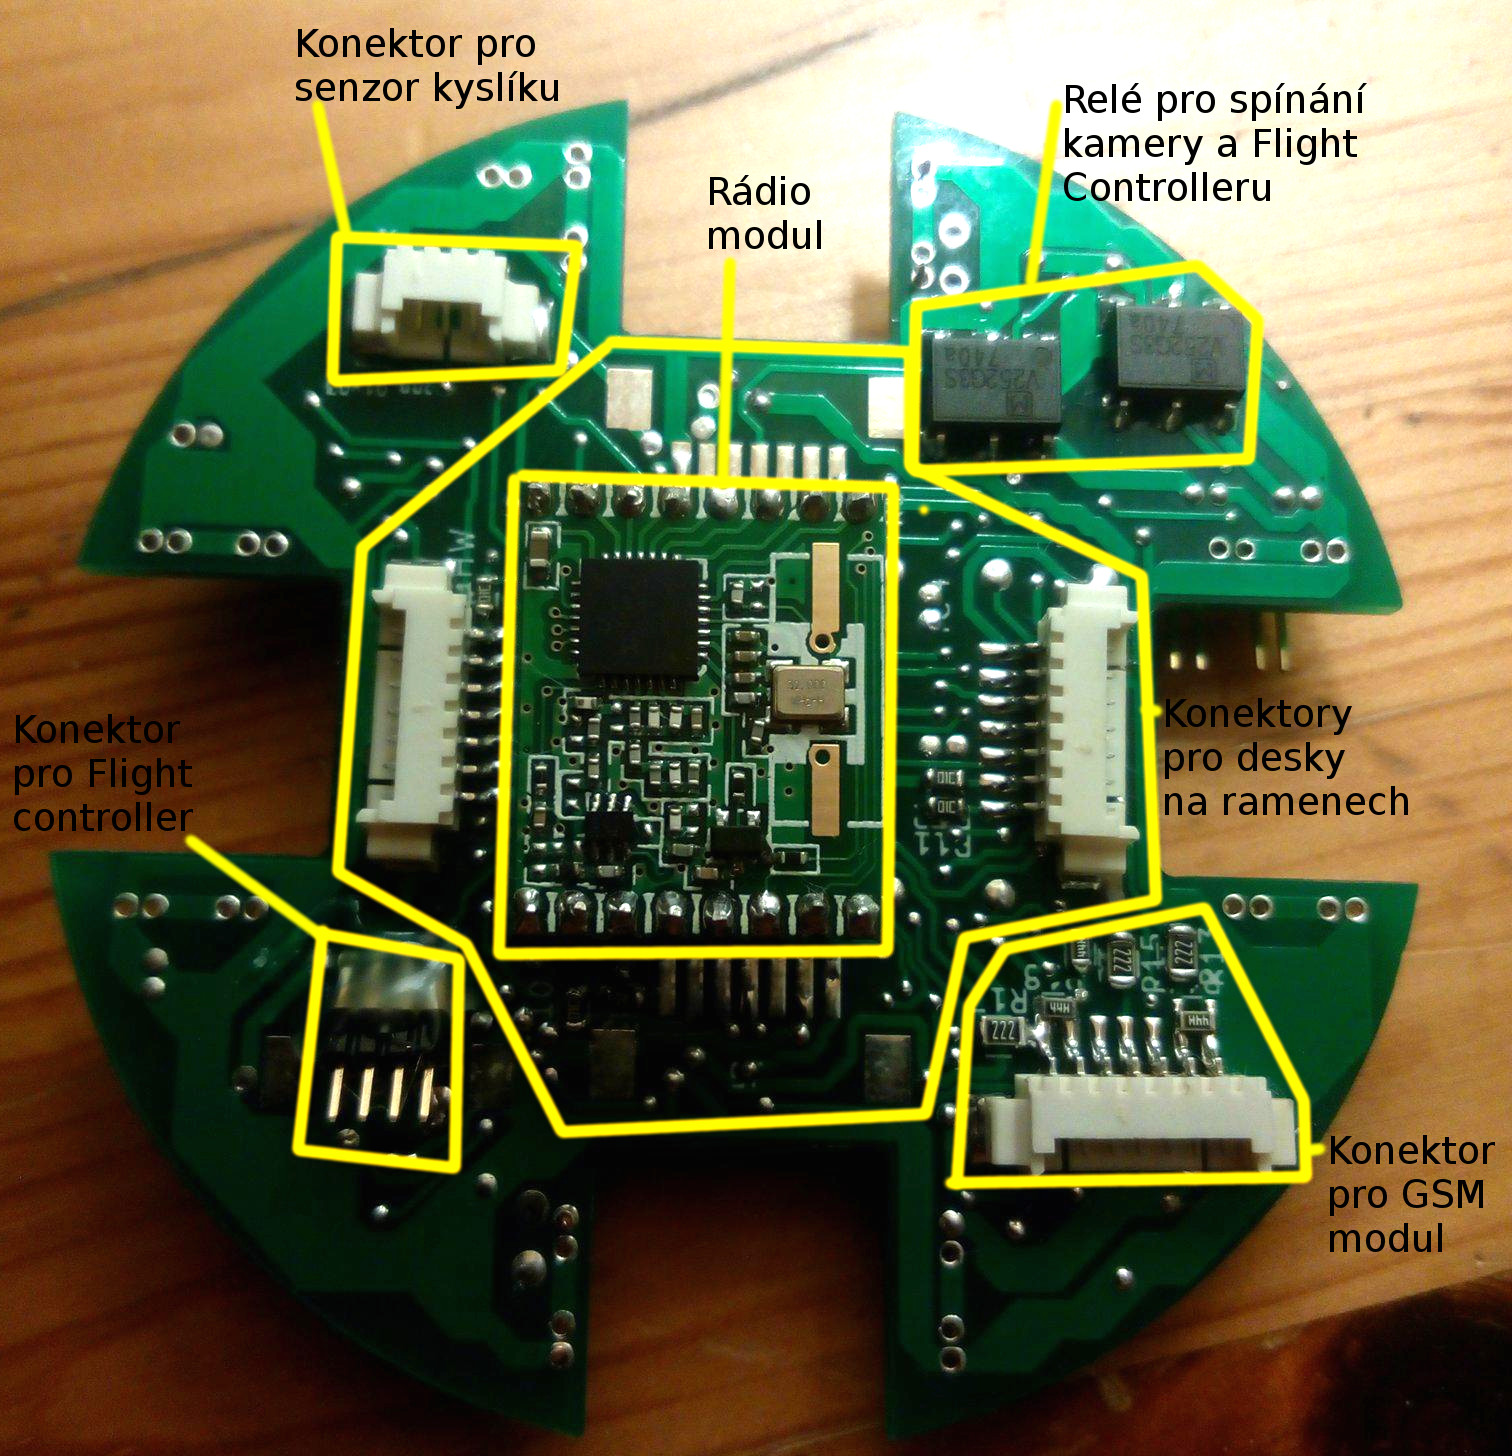
\includegraphics[width=400pt]{main1.jpg}
\end{figure}
\begin{figure}[H]
\centering
\caption{Řídící deska zdola, zdroj: Jakub Suchánek}
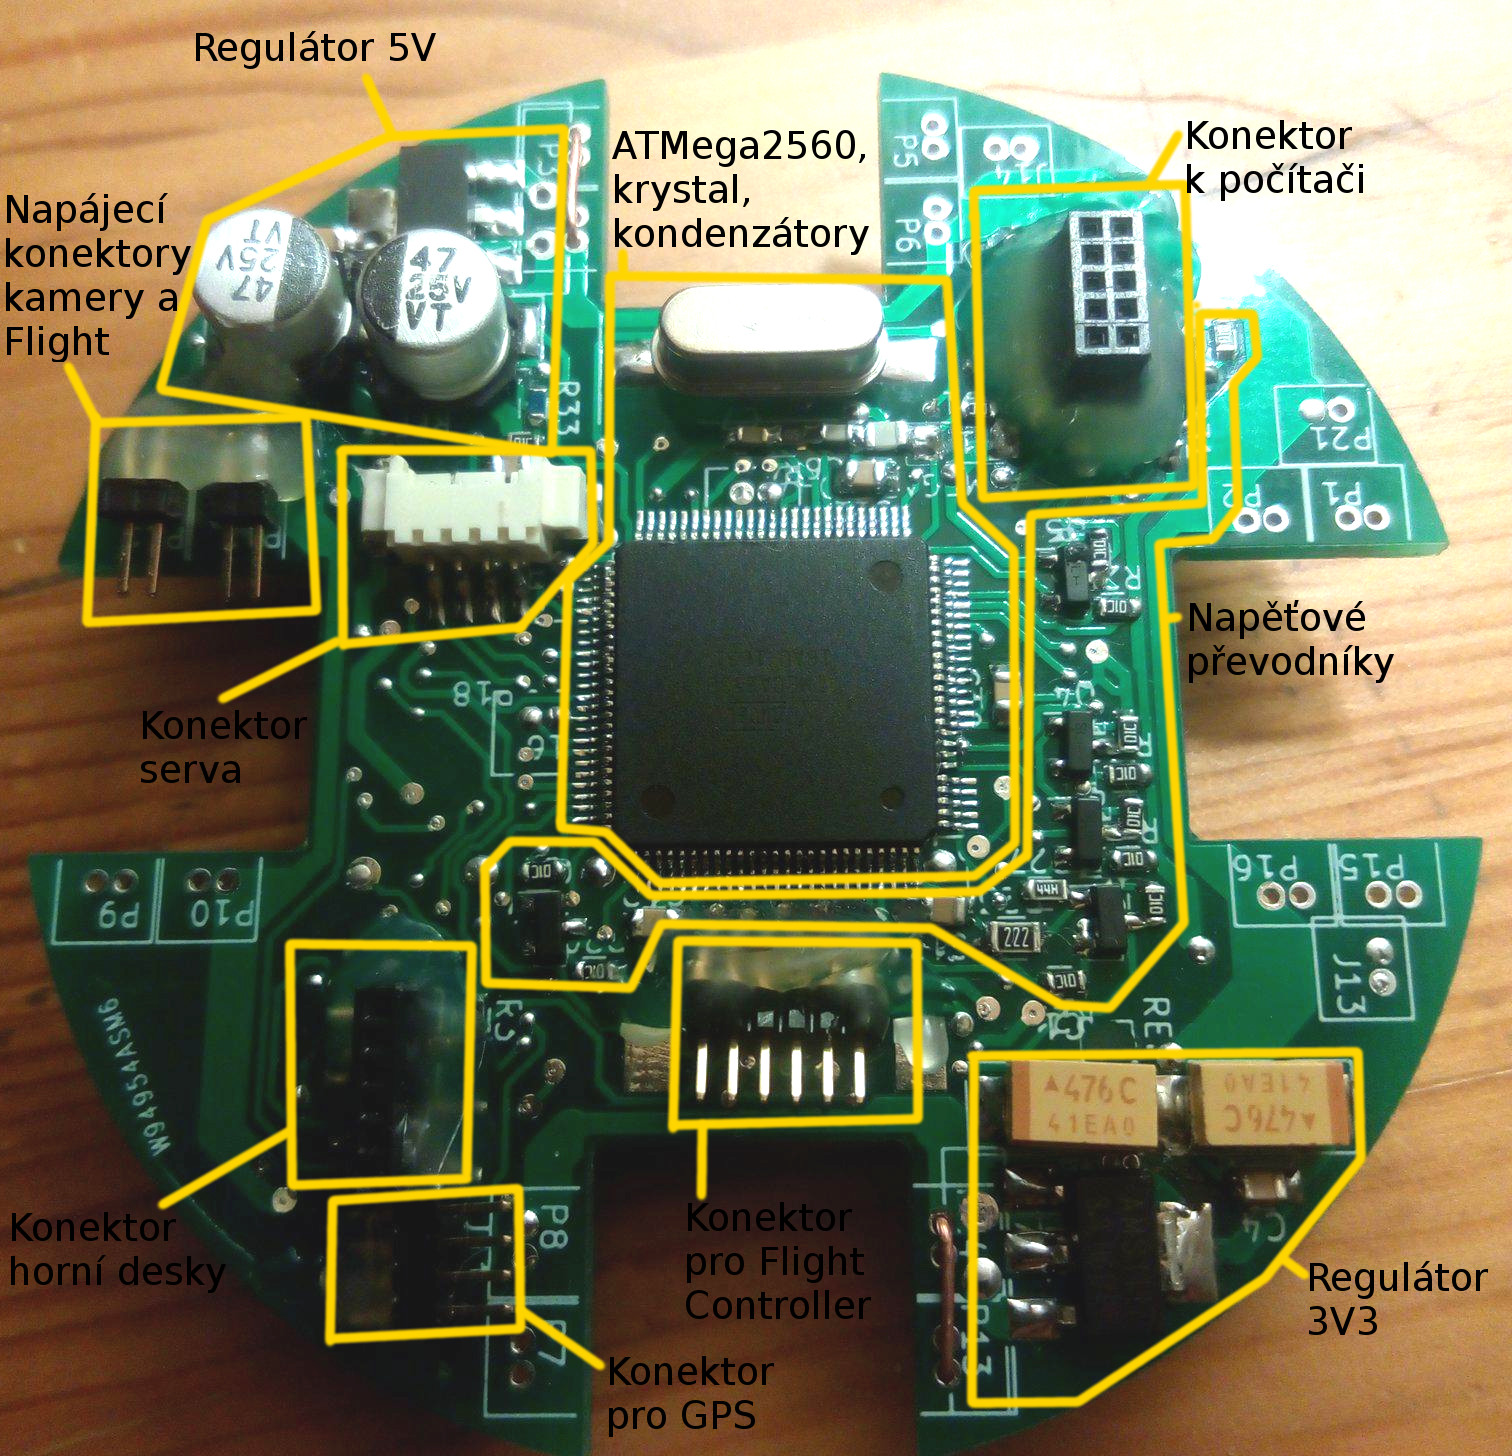
\includegraphics[width=400pt]{main2.jpg}
\end{figure}
\subsubsection{ATmega2560-16AU - mikrokontroler}
\paragraph{} Mikrokontroler vyvinutý společností Atmel, při 5V funguje s frekvencí krystalu až 16 MHz. Byl zvolen pro velké množství GPIO pinů, 4 sériové linky (USART) a dostatečně vysokou frekvenci časovače pro potřeby CanSatu.
\begin{figure}[H]
\caption{ATmega2560-16AU, zdroj: \href{https://www.microchip.com/_images/ics/medium-ATmega2560-TQFP-100.png}{Microchip}}
\centering
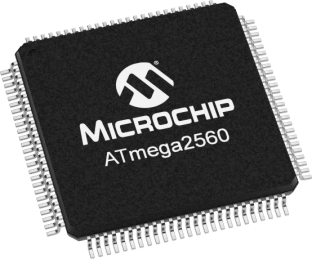
\includegraphics[width=200pt]{ATmega2560.png}
\end{figure}
\subsubsection{Regulace napětí}
\paragraph{} Využívá regulátory NCP1117, každý má vlastní přepínač. Napájení je rozvedeno kruhovými drahami, aby se minimalizovaly ztráty napětí.
\subsubsection{Napěťové převodníky}
\paragraph{} Založené na MOSFET tranzistoru bss138, který umožňuje propagaci nulového signálu mezi stranami, jedničkový signál doplní pull-up ke správnému napětí.
\subsubsection{Radiový vysílač}
Je používán vysílač RFM69HW, jelikož je to nejvýkonější vysílač této velikosti. Při výkonu 200mW jsme při přímé viditelnosti dosáhli 6,7 km.
\begin{figure}[H]
\caption{RFM69HW, zdroj: \href{http://www.hoperf.com/rf_transceiver/modules/RFM69HW.html}{HOPERF}}
\centering
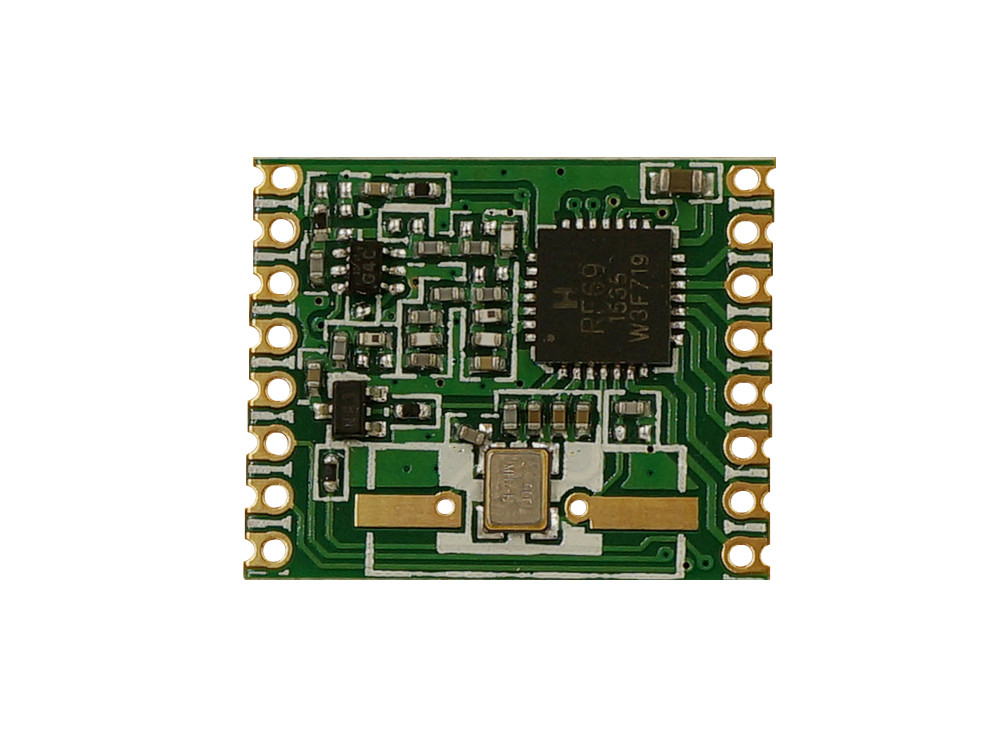
\includegraphics[width=200pt]{RFM69H.png}
\end{figure}
\subsection{Horní senzorová deska}
\paragraph{} Deska se senzory UV, vlhkosti a teploty, kompasu s akcelerometrem a signálový zesilovač pro senzor gamma záření. Senzory jsou umistěny zde, aby měřily vnější prostředí.
\begin{figure}[H]
\centering
\caption{Horní sensorová deska shora, zdroj: Jakub Suchánek}
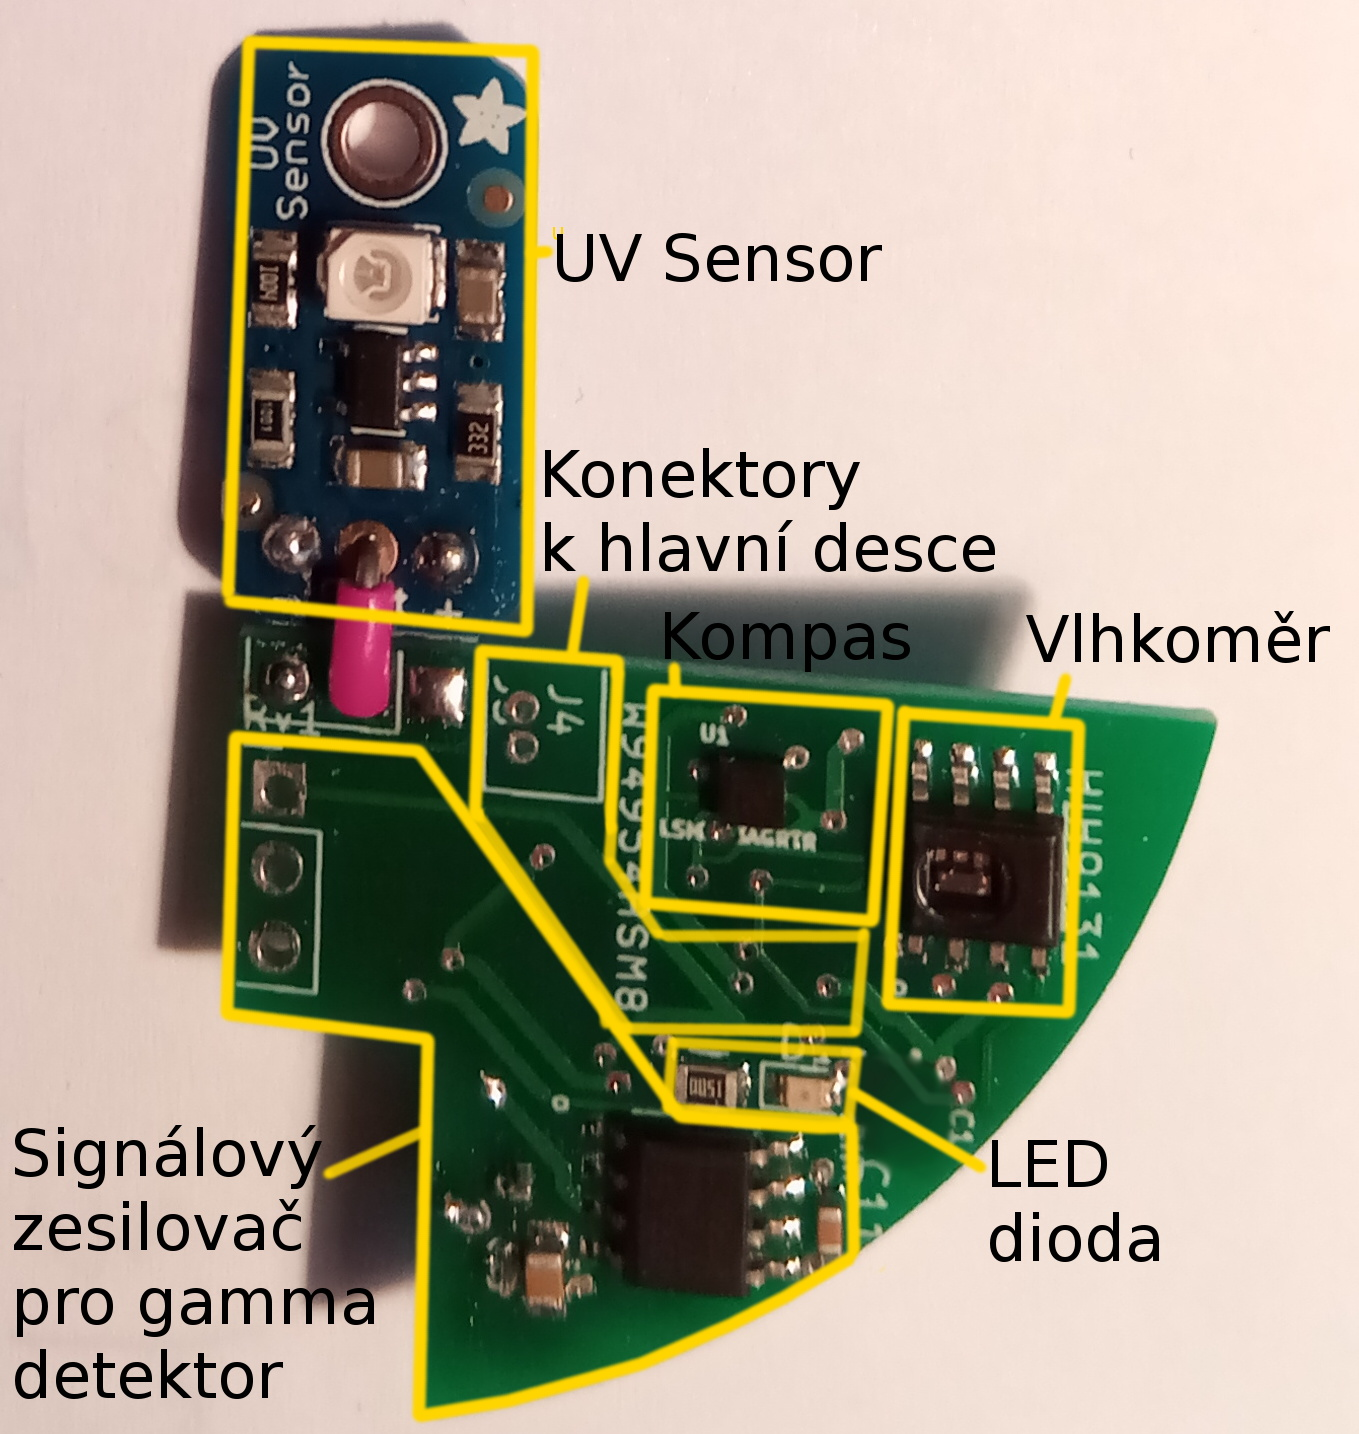
\includegraphics[width=250pt]{top1.jpg}
\end{figure}
\begin{figure}[H]
\centering
\caption{Horní sensorová deska zdola, zdroj: Jakub Suchánek}
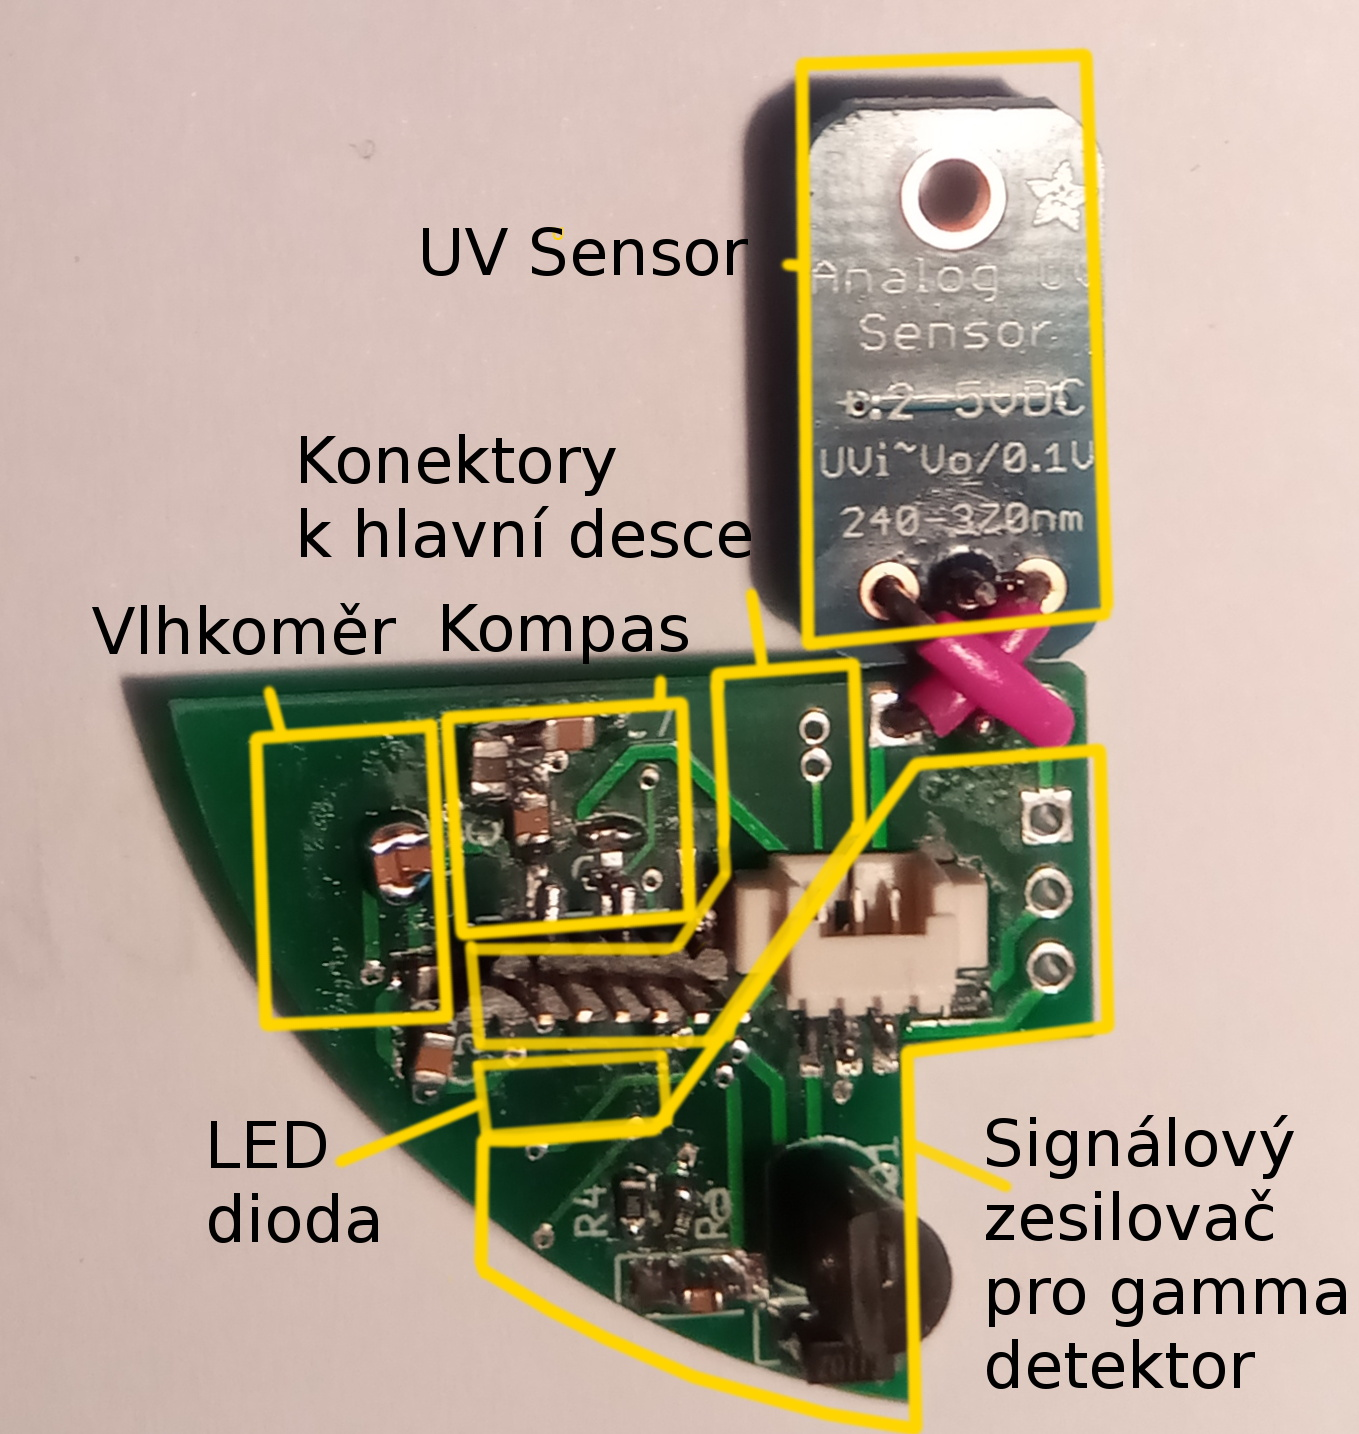
\includegraphics[width=250pt]{top2.jpg}
\end{figure}
\subsubsection{Tříosý magnetometr a akcelerometr: LSM303AGRTR}
\paragraph{} Ke zjišťování přesné polohy nám slouží magnetometr a akcelerometr v kombinaci s GPS anténou. Magnetometr používáme k měření velikosti a směru magnetické indukce Země, tudíž i úhlu, v jakém je Cansat nakloněn. Z akcelerometru vyhodnocujeme data o pohybu a zrychlení.
\begin{figure}[H]
\caption{LSM303AGRTR,zdroj: 
\href{http://uk.farnell.com/stmicroelectronics/lsm303agrtr/mems-3d-accelero-magneto-lga-12/dp/2664523RL}{Farnell}}
\centering
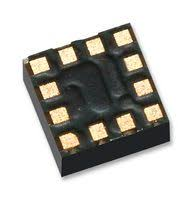
\includegraphics[width=150pt]{acc+mgn.jpg}
\end{figure}
\subsubsection{Senzor teploty a vlhkosti: HIH7130}
\paragraph{} Senzor HIH7130 je malý senzor určený na plošné spoje pro měření vzdušné teploty i vlhkosti. Získá přesnou hodnotu v rozmezí -40 až 100 stupňů Celsia.
\begin{figure}[H]
\caption{HIH7130, zdroj: 
\href{https://www.tme.eu/cz/details/hih7130-000-001/cidla-vlhkosti/honeywell/}{TME}}
\centering
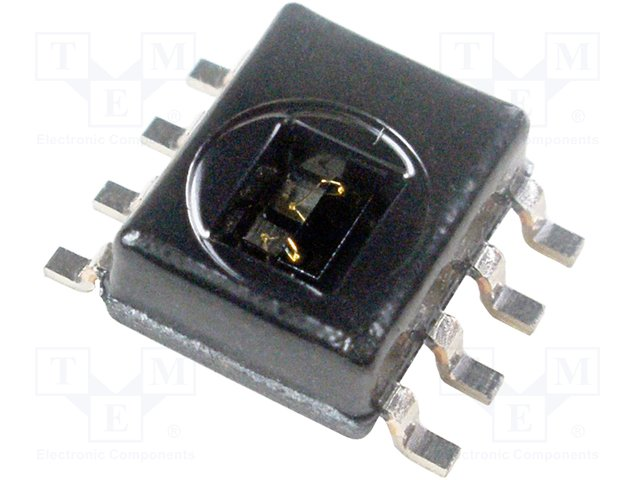
\includegraphics[width=150pt]{HIH7130.jpg}
\end{figure}
\subsubsection{UV senzor: Adafruit GUVA-S12SD}
\paragraph{} Senzor ultrafialového záření nám určí, zda-li na daném místě atmosféra nepropouští pro život nebezpečné UV záření. Funkce souvisí především s naším příběhem o detekci života na cizí planetě.
\begin{figure}[H]
\caption{Analog UV Light Sensor Breakout - GUVA-S12SD, zdroj: 
\href{https://www.adafruit.com/product/1918}{Adafruit}}
\centering
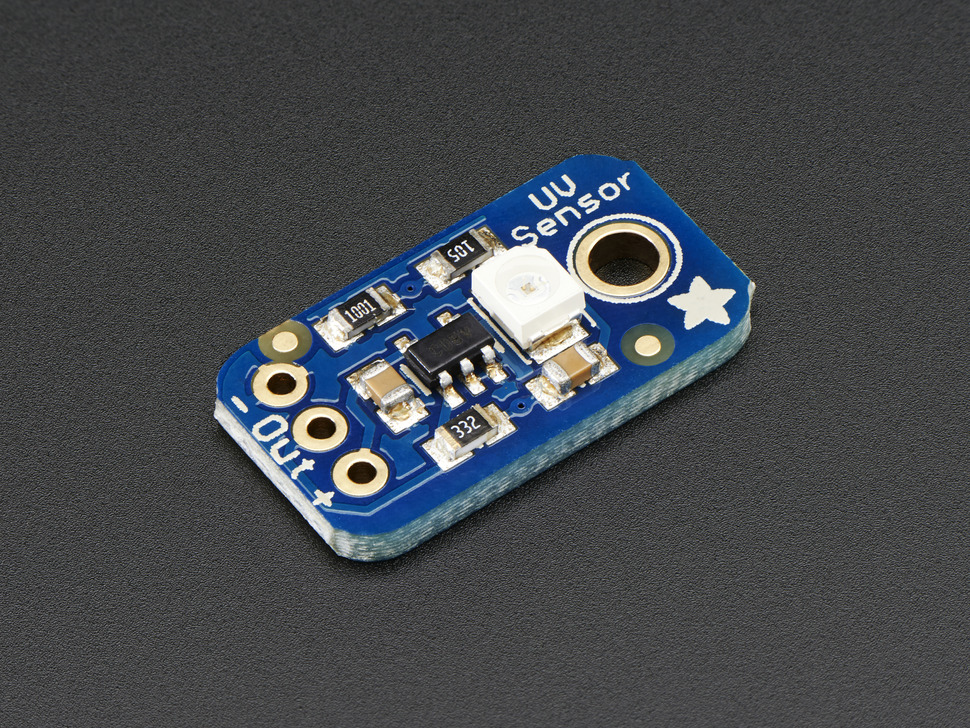
\includegraphics[width=200pt]{uv_senzor.jpg}
\end{figure}
\subsection{Desky na ramenech}
\paragraph{} Pro přesné měření vzdálenosti a stability při přistání jsou na ramenech namontovány desky se senzory vzdálenosti a zároveň se signalizačními LED diodami.
\begin{figure}[H]
\centering
\caption{Deska na ramenech, zdroj: Jakub Suchánek}
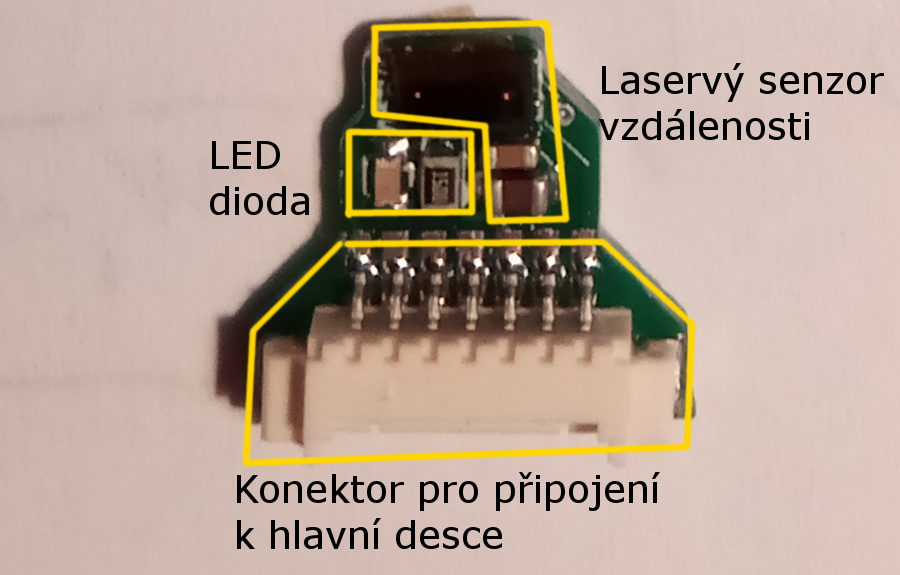
\includegraphics[width=200pt]{deska_rameno.jpg}
\end{figure}
\subsection{GSM modul: SIM808}
\paragraph{} GSM modul bude během letu odesílat nejrůznější data pomocí SMS zpráv. Zároveň se ozve našim fanouškům a napíše jim nejzajímavější informace o průběhu letu.
\begin{figure}[H]
\caption{SIM808, zdroj: 
\href{https://www.geeker.co.nz/accessories/gsm/sim808-gprs-gsm-gps-module.html}{GeekStudio}}
\centering
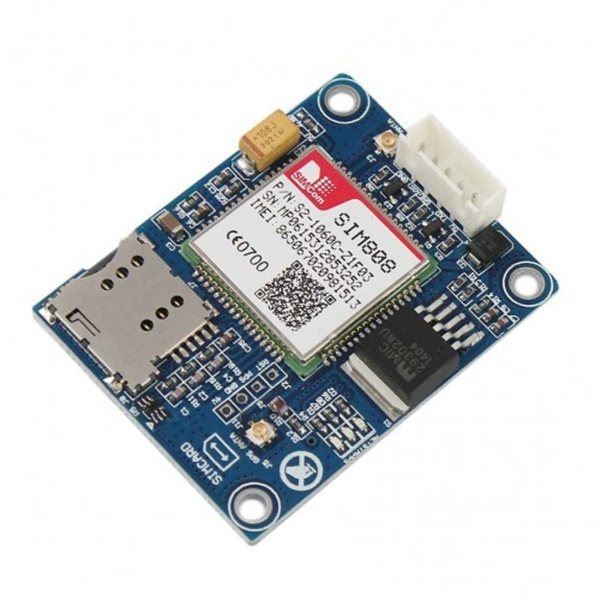
\includegraphics[width=150pt]{gsm.jpg}
\end{figure}
\subsection{Barometr: MPL3115A2}
\paragraph{} Barometr používáme na měření tlaku ve vzduchu a především pro určení nadmořské výšky.
\begin{figure}[H]
\caption{MPL3115A2, zdroj: 
\href{https://www.alza.cz/sparkfun-vyskomer-tlakomer-mpl3115a2-d3752617.htm?kampan=adpla_vyrobci_Komponenty_programovatelne-stavebnice_c_2o1_SEN112a_1003803&gclid=Cj0KCQjwhoLWBRD9ARIsADIRaxSYJAwB_WEpQJOK6349QjdAecPFdzJR4etdCMYp0Hs_YAw0_bWlqW8aAi1yEALw_wcB}{Alza}}
\centering
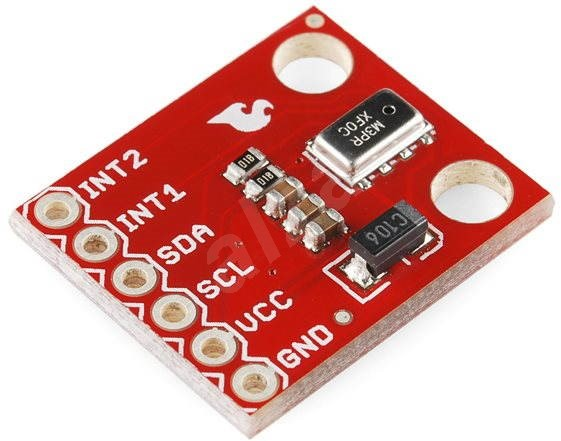
\includegraphics[width=150pt]{barometr.jpg}
\end{figure}
\subsection{Akumulátory: Turnigy Nano-Tech 200mAh 1S 35~70C}
\paragraph{} K napájení celého CanSatu používáme šestnáct lithium-polymerových baterií o kapacitě 200mAh.  Každá má pouze jeden článek s napětím 3,7V. Dvojice baterií zapojených sériově poskytuje dostatečné napětí 7,4V pro napájení motorů. Z těchto dvojic jsme složili čtyři sloupky nacházející se po obvodu našeho satelitu. Cílem tohoto neobvyklého řešení bylo ušetřit co nejvíce místa na ostatní komponenty.
\begin{figure}[H]
\centering
\caption{Turnigy Nano-Tech 200mAh 1S 35~70C, zdroj: 
\href{https://www.rotorama.cz/baterie/turnigy-nano-tech-200mah-1s-35-70c}{Rotorama}}
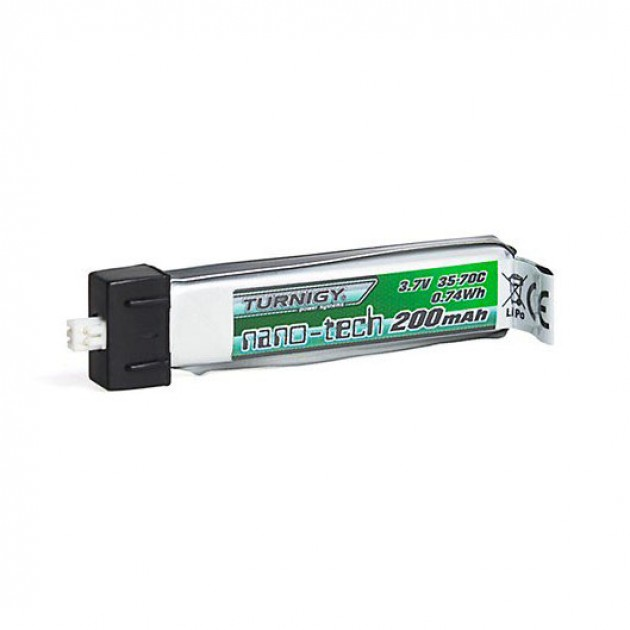
\includegraphics[width=200pt]{Baterie.jpg}
\end{figure}
\subsection{Motory: HGLRC Flame 1104 7500KV}
\paragraph{} O pohyb a především snížení dopadové rychlosti se starají čtyři výkonné motory s celkovým maximálním tahem 640 gramů.
\begin{figure}[H]
\centering
\caption{HGLRC Flame 1104 7500KV, zdroj: 
\href{https://www.rotorama.cz/motory/hglrc-flame-1104-7500kv}{Rotorama}}
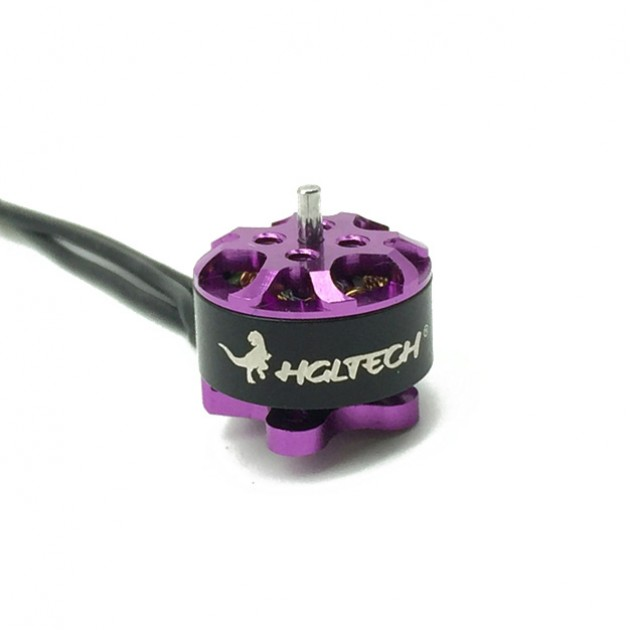
\includegraphics[width=200pt]{Motor.jpg}
\end{figure}
\subsection{Regulátory: DYS F18A 4in1 micro}
\paragraph{} K ovládání otáček motorů slouží čtyři ESC (Electric Speed Controller) umístěné na jedné desce. Zvládají proud až 18A a podporují i nejnovější protokol Dshot.
\begin{figure}[H]
\centering
\caption{DYS F18A 4in1 micro, zdroj: 
\href{https://www.rotorama.cz/regulatory/dys-f18a-4in1-micro}{Rotorama}}
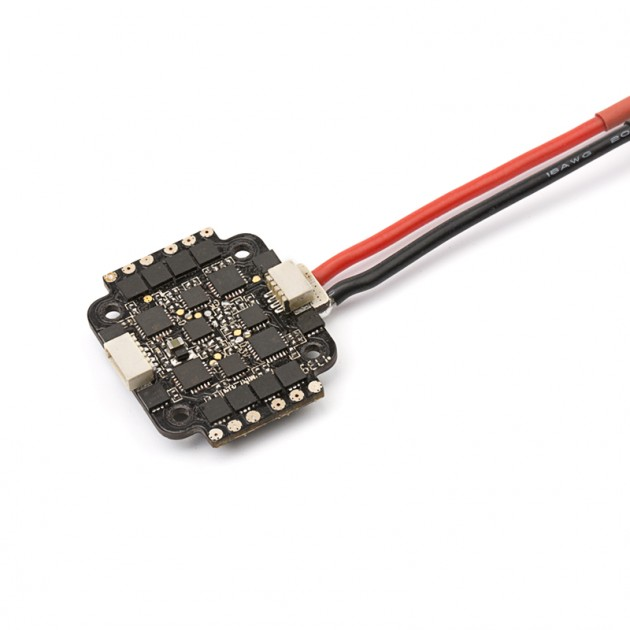
\includegraphics[width=200pt]{regulatory.jpg}
\end{figure}
\subsection{Řídící jednotka: SP Racing F3 Acro}
\paragraph{} Řídící jednotku (neboli Flight Controller) využíváme ke stabilizaci satelitu (dronu) za letu. Deska se používá především u závodních kvadrokoptér. Díky tomu má gyro a akcelerometr relativně vysokou obnovovací frekvenci až 4kHz, což nám zaručuje výbornou stabilizaci a plynulé pohyby satelitu. Jednotka komunikuje s naším mikroprocesorem pomocí osmi vstupních PWM pinů. Tyto piny jsou určené k přenosu informací o tom, jak se má dron pohybovat, například dle informací z GPS.
\begin{figure}[H]
\centering
\caption{SP Racing F3 Acro, zdroj: 
\href{http://team-legit.com/SP-Racing-F3-Flight-Controller-Acro-Standard-6DOF_p_660.html}{Team-Legit}}
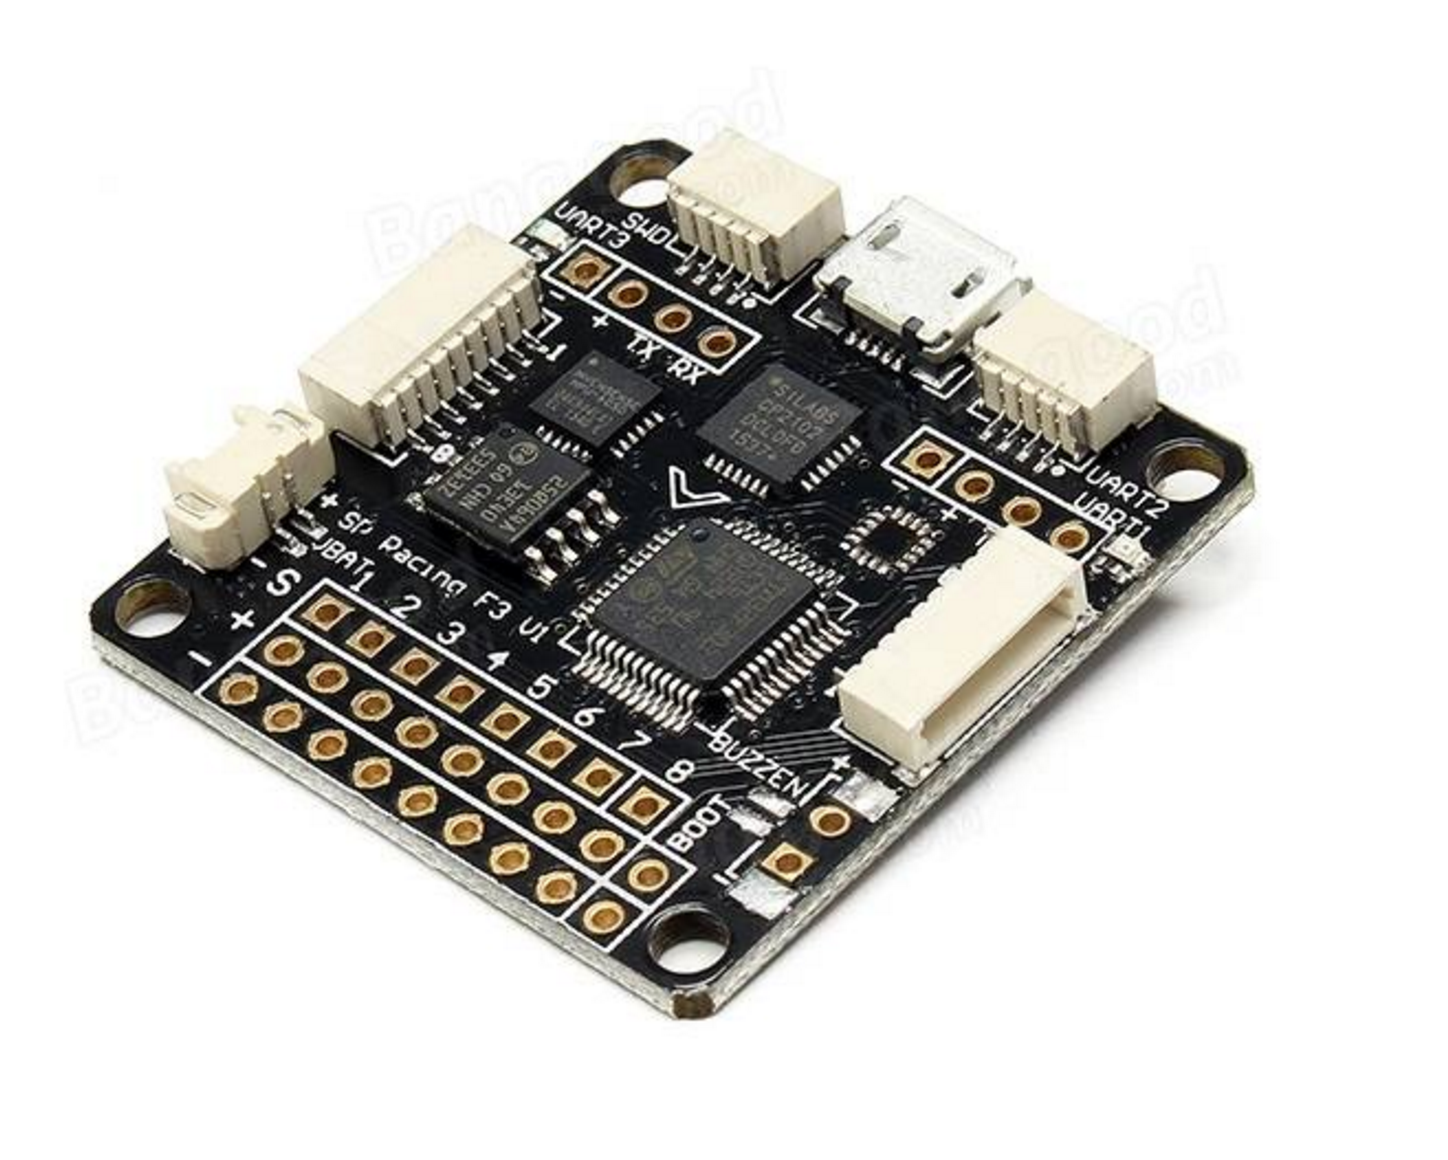
\includegraphics[width=200pt]{Jednotka.png}
\end{figure}
Obsahuje:
\begin{itemize}
\item STM32 CPU 32bit
\item MPU6050 gyro/acc
\end{itemize}
\subsection{Kamera s vysílačem: Eachine TX01}
\paragraph{} Tato kamera nám umožní snímat obraz ve slušném rozlišení a vysílat ho přímo na zem k našemu stanovišti s minimální latencí. Součástí je video vysílač o výkonu pouhých 25mW, jelikož legislativa v České republice zakazuje použít vyšší vyzařovací výkon. Pro správný přenos je využita všesměrová cirkulární anténa. 
\begin{figure}[H]
\centering
\caption{Kamera Eachine TX01, zdroj:
\href{https://www.rotorama.cz/fpv/eachine-tx01}{Rotorama}}
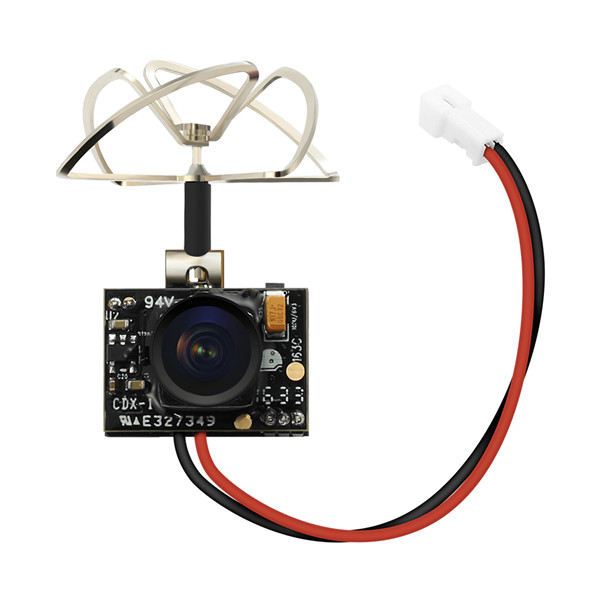
\includegraphics[width=200pt]{Kamera.jpg}
\end{figure}
\subsection{GPS modul: Ublox M8N}
\paragraph{} Modul používáme k přijímání GPS souřadnic, které jsou následně vyhodnocovány naším hlavním mikroprocesorem a ten vytvoří letový plán. Navíc jsou souřadnice zasílány na zem k našemu stanovišti, díky tomu máme přehled, kde se satelit nachází.
\begin{figure}[H]
\centering
\caption{GPS modul: Ublox M8N, zdroj: 
\href{https://alexnld.com/product/7m-8m-ublox-m8n-gps-module-for-apm-pixhawk-cc3d-naze32-f3-flight-control/}{AlexNLD}}
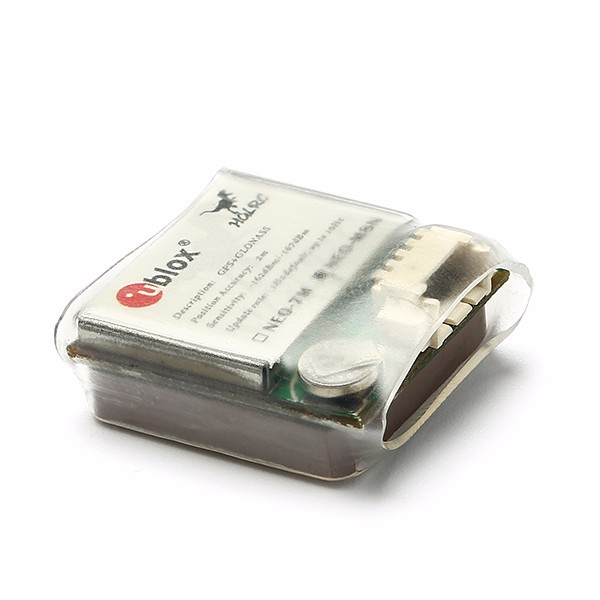
\includegraphics[width=200pt]{GPSmodul.jpg}
\end{figure}
\subsection{Čidlo gamma záření}
\paragraph{}Tento senzor je zkonstruován z fotodiody, jež je zastíněna neprůhledným materiálem, aby se zabránilo průchodu záření o nižších frekvencích než $\gamma$. Signál je nejprve zesílen přes tranzistor (jak je znázorněno ve schématu), který je společně s diodou umístěn v kovovém obalu za účelem eliminace rušení. Další stupeň je tvořen operačním zesilovačem již na plošném spoji.
\begin{figure}[H]
\centering
\caption{Zdroj:
\href{http://www.vk2zay.net/article/265}{Alan's lab}}
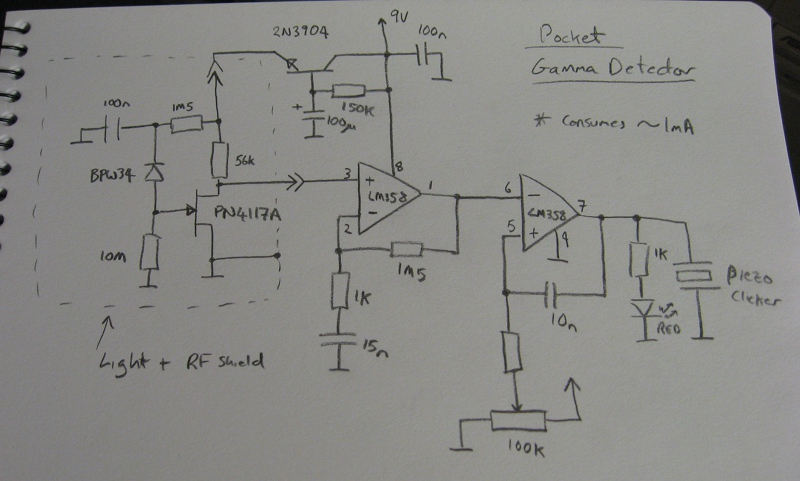
\includegraphics[width=200pt]{pd-gamma-counter-circuit.jpg}
\end{figure}
\subsection{Celkový seznam dílů:}
\begin{longtable}{L{6cm}L{3cm}L{3cm}L{3cm}}
Součástka               & V CanSatu & Cena       & Cena za kus \\
ATmega                  & 1         & 321,22Kč   & 321,22Kč    \\
Baterie                 & 16        & 1 424,00Kč & 89,00Kč     \\
bss138                  & 6         & 13,80Kč    & 2,30Kč      \\
čidlo vzdálenosti       & 4         & 558,83Kč   & 139,71Kč    \\
dioda                   & 1         & 3,97Kč     & 3,97Kč      \\
GSM modul               & 1         & 506,50Kč   & 506,50Kč    \\
hlavní vypínač          & 2         & 107,18Kč   & 53,59Kč     \\
J-FET                   & 1         & 76,51Kč    & 76,51Kč     \\
kamera, anténa, vysílač & 1         & 619,00Kč   & 619,00Kč    \\
kon 0,22 uF             & 2         & 5,83Kč     & 2,92Kč      \\
kon 0,8 uF              & 1         & 2,92Kč     & 2,92Kč      \\
kon 10 nF               & 1         & 1,23Kč     & 1,23Kč      \\
kon 10 uF               & 1         & 4,49Kč     & 4,49Kč      \\
kon 100 nF              & 15        & 33,40Kč    & 2,23Kč      \\
kon 100 nF              & 1         & 4,74Kč     & 4,74Kč      \\
kon 100 uF              & 2         & 26,33Kč    & 13,16Kč     \\
kon 10nF                & 1         & 2,64Kč     & 2,64Kč      \\
kon 22pF                & 1         & 2,38Kč     & 2,38Kč      \\
kon 4,7 uF              & 4         & 83,25Kč    & 20,81Kč     \\
kon 47 uF               & 4         & 27,39Kč    & 6,85Kč      \\
kon. 20 pF              & 2         & 5,28Kč     & 2,64Kč      \\
konektor 2x5            & 1         & 1,60 Kč    & 1,60 Kč     \\
konektor 2x5            & 1         & 1,42Kč     & 1,42Kč      \\
krystal                 & 1         & 9,47Kč     & 9,47Kč      \\
LED cervená             & 3         & 25,26Kč    & 8,42Kč      \\
LED zelená              & 2         & 30,06Kč    & 15,03Kč     \\
magnetometr             & 1         & 69,70Kč    & 69,70Kč     \\
Motory                  & 4         & 1 156,00Kč & 289,00Kč    \\
NPN                     & 1         & 10,53Kč    & 10,53Kč     \\
operační zesilovač      & 1         & 10,81Kč    & 10,81Kč     \\
PIN dioda               & 1         & 31,91Kč    & 31,91Kč     \\
plošné spoje            & 1         & 225,60Kč   & 225,60Kč    \\
potentiometer 100k      & 1         & 22,00Kč    & 22,00Kč     \\
regulátor 3V3           & 1         & 49,00Kč    & 49,00Kč     \\
regulátor 5V            & 1         & 11,86Kč    & 11,86Kč     \\
regulátory              & 1         & 799,00Kč   & 799,00Kč    \\
relé                    & 2         & 592,88Kč   & 296,44Kč    \\
rez 10k                 & 23        & 131,08Kč   & 5,70Kč      \\
rez 10M                 & 1         & 2,64Kč     & 2,64Kč      \\
rez 150                 & 5         & 13,19Kč    & 2,64Kč      \\
rez 150k                & 1         & 8,70Kč     & 8,70Kč      \\
rez 1k                  & 2         & 5,28Kč     & 2,64Kč      \\
rez 1m                  & 1         & 8,70Kč     & 8,70Kč      \\
rez 1M5                 & 1         & 2,64Kč     & 2,64Kč      \\
rez 1M5                 & 1         & 3,16Kč     & 3,16Kč      \\
rez 2k                  & 2         & 5,28Kč     & 2,64Kč      \\
rez 2k2                 & 4         & 10,55Kč    & 2,64Kč      \\
rez 2k8                 & 4         & 10,55Kč    & 2,64Kč      \\
rez 4k7                 & 3         & 10,31Kč    & 3,44Kč      \\
rez 56k                 & 1         & 2,92Kč     & 2,92Kč      \\
RFM69HW-433S2           & 1         & 89,76 Kč   & 89,76 Kč    \\
Rotory (vrtulky)        & 1         & 41,00Kč    & 41,00Kč     \\
řídící jednotka         & 1         & 329,00Kč   & 329,00Kč    \\
senzor CO2              & 1         & 662,27Kč   & 662,27Kč    \\
senzor O2               & 0         & 0,00Kč     & 1 553,45Kč  \\
Servo                   & 1         & 24,00Kč    & 24,00Kč     \\
sig. konektory          & 1         & 2,66 Kč    & 2,66 Kč     \\
sig. konektory          & 1         & 8,07Kč     & 8,07Kč      \\
sig. konektory          & 9         & 114,48 Kč  & 12,72 Kč    \\
sig. konektory          & 9         & 32,00 Kč   & 3,56 Kč     \\
sig. konektory          & 122       & 25,17 Kč   & 0,21 Kč     \\
sig. konektory          & 21        & 28,19 Kč   & 1,34 Kč     \\
sig. konektory          & 21        & 74,52 Kč   & 3,55 Kč     \\
sig. konektory          & 2         & 28,12 Kč   & 14,06 Kč    \\
sig. konektory          & 2         & 5,27 Kč    & 2,63 Kč     \\
sig. konektory          & 2         & 5,11 Kč    & 2,56 Kč     \\
sig. konektory          & 2         & 16,88 Kč   & 8,44 Kč     \\
UV senzor               & 1         & 171,30Kč   & 171,30Kč    \\
vlhkoměr                & 1         & 211,57Kč   & 211,57Kč    \\
tlakový senzor          & 1         & 439,00Kč   & 439,00Kč    \\
gps                     & 1         & 298,00Kč   & 298,00Kč    \\
uhlíkové profily		& 0,3	    & 103,00Kč	 & 30,90Kč	   \\
konstrukce	            & 1     	& 80,00Kč	 & 80,00Kč     \\
\end{longtable} \newpage
\section{Pozemní hardwarové vybavení}
\subsection{Desinfekční komora}
\paragraph{} UV trubka je doma vyrobený zdroj UV záření z 13 watové UVC zářivky a zbytků kuchyňského světla, stíněný okapovou rourou. Mimo generaci UV záření o vlnové délce 253,7 nm, které rozbíjí jádra buněk živých organismů, také vytváří molekuly \ce{O3}. Je nutná pro předletovou dekontaminaci CanSatu.
\begin{figure}[!h]
\centering
\caption{Mutace způsobená UV zářením, zdroj: \href{https://earthobservatory.nasa.gov/Features/UVB/}{NASA/David Herring}}
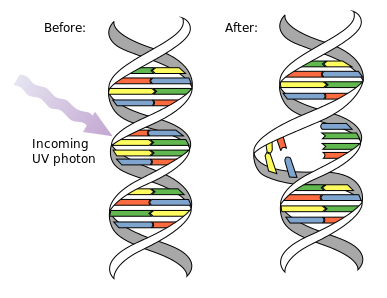
\includegraphics[width=400pt]{UVCmutation.png}
\end{figure}
\begin{figure}[!h]
\centering
\caption{UV trubka, zdroj: Patrik Novotný}
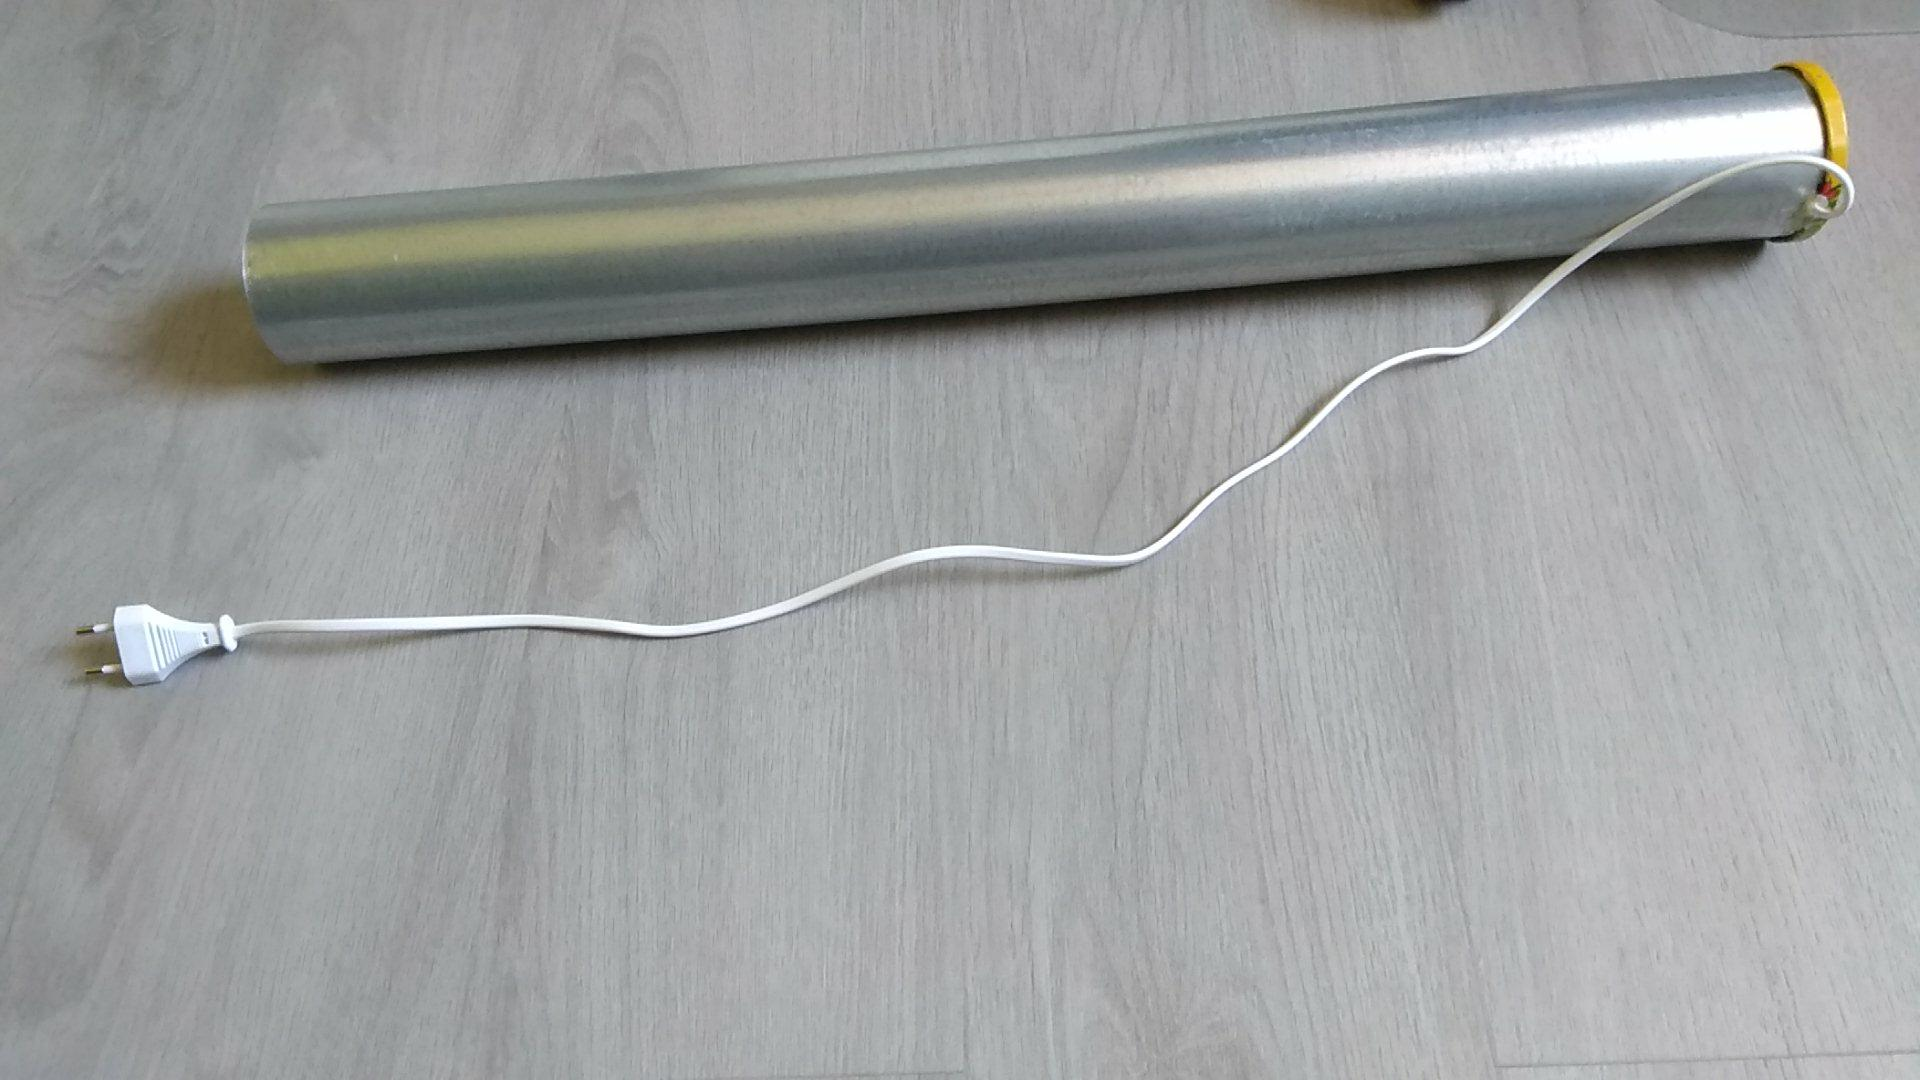
\includegraphics[width=400pt]{uv_lampa.jpg}
\end{figure}
\subsection{Anténa}
\paragraph{}Pro pozemní příjem signálu na 434 MHz používáme anténu Yagi vlastní výroby zkonstruovanou z hliníkových trubek.Zvolili jsme verzi o devíti prvcích (včetně reflektoru), kdy stále není extrémně neskladná, ale již poskytne dostatečný zisk 14dB a rádius 41° při ztrátě 3dB. Dále je snadno demontovatelná na jednotlivé prvky, což výrazně usnadňuje logistiku.
\section{Softwarové vybavení}
\paragraph{} Rádi bychom upozornili na to, že nejen všechen náš software, ale i tato správa a modely CanSatu, obecně všechen kód, má open source licenci.
\begin{figure}[!h]
\centering
\caption{Flow chart , zdroj: Jakub Suchánek}
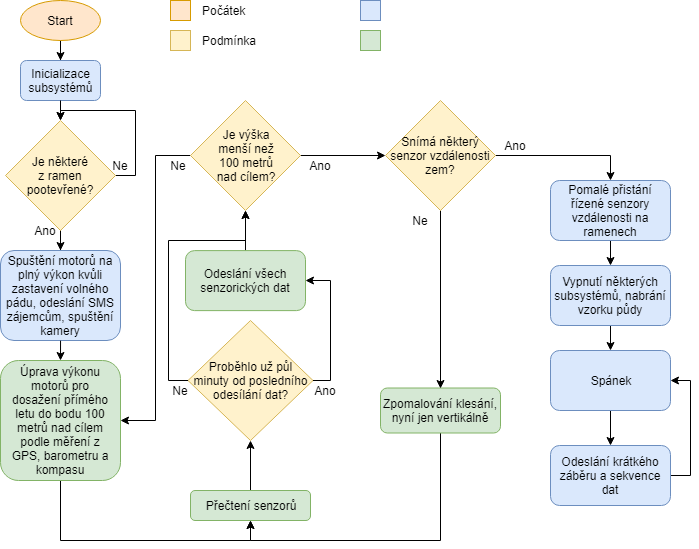
\includegraphics[width=400pt]{Software.png}
\end{figure}
\paragraph{} Veškerý software je napsaný v jazyce Arduino založeném na C++. Využíváme mnoho knihoven, za všechny děkujeme autorům. Software je veřejný na našem \href{https://github.com/suchanekj/CanSatGOSA}{gitu}.
\section{Pozemní softwarové vybavení}
\paragraph{} Na pozemní stanici bude Arduino připojené do počítače s přijímací anténou a zároveň poběží na počítači program v \href{https://processing.org/}{Processingu}, což je vývojové prostředí založené na jazyce Java s mnoha knihovnami. Právě jednu z nich používáme na komunikaci s Arduinem.
\paragraph{} Na Arduinu je nahraný program \href{https://github.com/suchanekj/CanSatGOSA/blob/master/Code/GroundStation/GroundStation.ino}{GroundStation.ino}. Tento jednoduchý program pouze vypisuje na Sériový port přijatá data spolu s dalšími informacemi v hranatých závorkách (pořadí přijaté zprávy, ID odesílatele).
\paragraph{} Program  \href{https://github.com/suchanekj/CanSatGOSA/blob/master/Code/GroundStation/GroundStationToWeb.pde}{GroundStationToWeb.pde} naslouchá na sériovém portu, který je zrovna zapojený, a veškerá přijatá data zapisuje do souboru CanSatData.txt (s datem a časem vytvoření souboru v názvu), uloženém lokálně přímo u programu spolu s časem zápisu. Kromě lokálního ukládání komunikace se data odesílají na web. Program sestaví url, která bude obsahovat parametry s daty k uložení a otevře spojení pomocí této url. Program dostane odpověď, jež se zapíše do souboru CanSatHTMLResponse.txt (s datem a časem vytvoření souboru v názvu), umístěného stejně jako výše zmíněný textový soubor.

\section{Problémy}
\paragraph{} Jedním z velkých problémů, který nás postihl, bylo to, že náš plošný spoj nefungoval. Jakub Suchánek tudíž navštívil Robotárnu v Brně a s pomocí osciloskopu zjistil, že na plošném spoji byla připájena dioda v závěrném směru. Po jejím otočení spoj funguje.
\paragraph{} Již od semifinále víme, že limit pro evropské kolo je vyšší než pro kolo národní, že tudíž nebudeme moci osadit \ce{O2} senzor.
\paragraph{} Menším problémem byl spor se společností Disney. Když jsme streamovali pájení součástek na plošný spoj, tak nám byl přenos po upozornění od společnosti Disney smazán společností Youtube pro porušení autorských práv. Jako podkladovou hudbu jsme použili Novosvětskou symfonii od Antonína Dvořáka nahranou začátkem minulého století, nyní již ve veřejném vlastnictví. Ukázalo se, že oznámení učinil bot, který našel shodu v pár vteřinách nahrávky, ač jsme ji měli ze zdroje hudby s vypršelou licencí. Tento spor jsme dále neřešili, protože na naší nahrávce stejně nebylo mnoho zajímavého vidět, a video z pájení tedy není veřejné.
\paragraph{} Problémy jsme dále měli s instalací baterií do CanSatu, kde je velice málo místa. Při dotyku jednoho z osmi kabelů (máme 4x4 články) došlo ke zkratu. Problém jsme vyřešili přidáním konektorů na konce čtyřčlánků.
\paragraph{} Dalším poměrně velkým problémem byl střet se sedlákem během testu nouzových systémů - tz. chytání CanSatu do plachty pro případ selhání motorů. Test jsme prováděli na poli, kde běžně vypouštějí modeláři svá letadélka. Pan zemědělec si myslel, že naší skupinu kdysi již vyháněl, a proto nám traktorem zablokoval auta a chtěl volat policii. Snaha kapitána Patrika Novotného o diplomatické jednání se minula účinkem. Až asertivní styl jednání PR a HR odborníka Jana Janouška pomohl tomu, že na nás daný muž přestal útočit a umožnil nám pole opustit a přesunout se na jiné místo. S jiným takto útočným jednáním jsme se naštěstí již nesetkali.
\section{Výhled do budoucna}
Postoupíme-li do evropského kola soutěže, osadíme satelit dalšími čidly, díky vyššímu povolenému limitu, který činí 500\EUR. Již nyní máme čidlo \ce{O2} za 1200 Kč, jež nemůžeme kvůli cenovému limitu pro Českou republiku osadit. Také pravděpodoně koupíme nové baterie z důvodu větší kapacity. Mimo výše zmíněného a mimo úprav ve vedení kabílků nezvažujeme další úpravy. V případě postupu do evropského kola nám firma EPSON slíbila zajistit vystoupení v pořadu typu Snídaně s Novou, a tím i představit veřejnosti sebe, náš tým i celou soutěž ESA CanSat. Ať již uspějeme na jakkékoli úrovni či nikoliv, je zřejmé, že nás příprava CanSatu velmi bavila. Proto jsme se rozhodli, že se zúčastníme i mezinárodní soutěže pro studenty vysokých škol \href{http://www.cansatcompetition.com/}{CanSat Competition}.
\section{Rozpočet}
\paragraph{} V rozpočtu jsou zařazeny naše celkové příjmy a výdaje. Neuvádíme zapůjčené nebo využité vnější vybavení, za ty děkujeme sponzorům níže, zde jsou uvedena pouze čistá finanční data. Prováděli jsme nákupy v dolarech a eurech, tyto nákupy jsme převedli dle údajů v ČNB ke dni nákupu. Celkové účetnitnicví je platné k 12. dubnu 2018.
\subsection {Výdaje}
\paragraph{} Vnitřní vybavení CanSatu:
 \begin{tabbing}
    Název ~~~~\= Cena ~~~~
    \= 34 \kill
    \bfseries  Název\>\>
    \bfseries Cena\>\\
    Pohonné systémy \>\>1526,00 Kč\\
    Baterie \>\>1424,00 Kč\\
    Mikroelektronika \>\>6749,32Kč Kč\\
    Konstrukce \>\>110,90 Kč\\\\
    Celkem \>\>9810,22 Kč\\
    \end{tabbing}
Kompletní seznam dílů naleznete v kapitole hardwarové vybavení, ta je však spíše stylizovaná na jejich využití nikoli rozpočtovou stránku. Díly darované s výraznou slevou společností Rotorama (Kamera a motory) účtujeme dle cen obchodu Banggood v souladu s pravidly soutěže.
\paragraph{} Výdaje mimo satelit:
 \begin{tabbing}
    Název ~~~~\= Cena ~~~~
    \= 34 \kill
    \bfseries  Název\>\>
    \bfseries Cena\>\\
    Mikiny \>\>1253,00 Kč\\
    Přijímací stanice \>\>304,00 Kč\\
    Díly Ev. kolo \>\>1283,84 Kč\\
    Doprava \>\>2281,84 Kč\\
    Ostatní výdaje \>\>5058,52 Kč\\\\
    Celkem \>\>10181,20 Kč\\
    \end{tabbing}
\paragraph{} Do položky ostatní výdaje patří jízdné do Brna a zpět, když Jakub Suchánek řešil na Robotárně Helceletova problémy našeho plošného spoje. Dále doprava dílů a zničené či záložní součástky.
\subsection {Příjmy}
\paragraph{} Dary našich podporovatelů:
 \begin{tabbing}
    Název ~~~~\= Cena ~~~~
    \= 34 \kill
    \bfseries  Název\>\>
    \bfseries Cena\>\\
    Epson \>\>\textbf{\EUR{300}}\\
    KPGO \>\>12 079.56 Kč\\
    Rotorama \>\>1283.84 Kč\\
    TUL - CXI \>\>400 Kč\\
    PCBWay \>\>20 \$\\\\
    Celkem \>\>22 090.76 Kč\\
    \end{tabbing}
\paragraph{} Tato tabulka si zaslouží delší vysvětlení - EPSON, náš generální partner, nám poskytl přímo daný obnos peněz. PCBWay a Rotoramu poskytly slevu ze zakoupených dílů - ta snižuje položku ostatní výdaje, tudíž nesnižuje cenu dílů vyúčtovaných v CanSatu. Technická univerzita Liberec - CXI nám vytiskla dvě verze našeho CanSatu, jejichž cenu jsme dle ceny materiálu odhadli na 400 Kč. Všechny zbývající náklady velkoryse zaplatil spolek KPGO. O našich sponzorech se více dočtete v další kapitole. Hodnotu výdajů lze také vyjádřit jako:
\paragraph{} Celkové příjmy = Výdaje celkem + Slevy a dary (=TUL-CXI + Rotorama + PCBWay)
\section{Cíle}
\begin{tabular}{|c|c|c|c|c|}
\hline
     Požadavek & Priorita & Analýza & Inspekce & Testování \\
\hline
     Hmotnost & Povinné & \tick & \tick & \\
\hline
     Cena & Povinné & \tick & \tick & \\
\hline
     Rozměry & Povinné & \tick & \tick & \\
\hline
     Let & Povinné & \tick & &\tick \\
\hline
     Telemetrické spojení & Povinné & \tick & &\tick\\
\hline
     GPS systém & Nepovinné & \tick & & \tick\\
\hline
     Řízený let & Nepovinné & \tick & & 15.4. v rámci komplexních testů \\
\hline
     Detekce života & Nepovinné & \tick & \tick & \tick \\
\hline
     Přenos videa & Nepovinné & \tick & & \tick \\
\hline
     GSM přenos & Nepovinné & \tick & &15.4. v rámci komplexních testů \\
\hline
     Detekce UV záření & Nepovinné & \tick & & \tick\\
\hline
\end{tabular}
\paragraph{} Vysvětlení tabulky: Dělení na povinné a nepovinné určujeme dle prepozic soutěže. Analýza znamená teoretický rozbor věci. Inspekce znamená, že jsme změřili fyzikální podstavu věci. Testování znamená, že daný úkol byl splněn a provedení daného úkolu je funkční.
\section{Poděkování podporovatelům}
\subsection{Sponzoři}
\paragraph{} Nejprve bychom rádi poděkovali těm, kteří nás podpořili finančně. V prvé řadě děkujeme našemu generálnímu partneru, firmě EPSON, která nám darovala roll-up a vytiskla blueprinty, v případě postupu do evropského kola nám zajistí širokou publicitu - výstup z finále přes PR agenturu Bison \& Rose a účast pořadu typu Snídaně s Novou s cílem popularizovat náš projekt i celou soutěž, případně krátký dokumentární film o soutěži.  Dále děkujeme společnostem Rotorama a PCBWay, které nám poskytly slevy ze svých výrobků. Velký dík patří Klubu přátel Gymnázia Opatov, který nám poskytl bezúročnou půjčku na samotný vývoj CanSatu, kterou jsme částečně vrátili z peněz sponzorů a zbytek nám byl převeden na dar. KPGO nám též poskytl právní záštitu. Další poděkování patří Jiřímu Šefkovi z Ústavu pro nanomateriály, pokročilé technologie a inovace z Technické univerzity v Liberci, který nám vytiskl dvě verze CanSatu (včetně finální) na tamních špičkových 3D tiskárnách. Poslední díky patří Jakubovi Rozehnalovi, řediteli, Hvězdárny a Planetária Praha, který nám zapůjčil nutné vybavení.
\begin{figure}[H]
\centering
\caption{Logo Epson, zdroj: 
\href{https://www.epson.cz}{Epson}}

\includegraphics[width=240pt]{epson.png}
\end{figure}
\begin{figure}[H]
\centering
\caption{Logo Gymnázia Opatov, zdroj: 
\href{http://gymnazium-opatov.cz}{Gymnazium Opatov}}

\includegraphics[width=240pt]{LogoGO.png}
\end{figure}
\paragraph{} Zde mělo být logo KPGO neboli Klubu přítel Gymnázia Opatov, jelikož však ten logo nemá, uveřejňujeme logo Gymnázia Opatov, s nímž jsou aktivity KPGO úzce spjaty.
\begin{figure}[H]
\centering
\caption{Logo Rotorama, zdroj: 
\href{https://www.rotorama.cz}{Rotorama}}

\includegraphics[width=240pt]{rotorama.png}
\end{figure}
\begin{figure}[H]
\centering
\caption{Logo TUL-CXI, zdroj: 
\href{http://cxi.tul.cz}{TUL-CXI}}

\includegraphics[width=240pt]{tul.png}
\end{figure}
\begin{figure}[H]
\centering
\caption{Logo PCBWay, zdroj: 
\href{http://pcbway.com}{PCBWay}}

\includegraphics[width=240pt]{pcbway.png}
\end{figure}
\begin{figure}[H]
\centering
\caption{Logo Planetária Praha, zdroj: 
\href{http://www.planetarium.cz}{Planetarium Praha}}

\includegraphics[width=200pt]{planet.png}
\end{figure}
\paragraph{} Jako poděkování za podporu jsme umístili loga našich sponzorů na svá trička, která navrhl Lukáš Vőlfl. Pořídili jsme si též mikiny a kšiltovky s logem GOSA, čímž vzniká celý set poutající pozornost na naše sponzory.
\begin{figure}[!h]
\centering
\caption{Vzor mikiny, zdroj Lukáš Vőlfl}
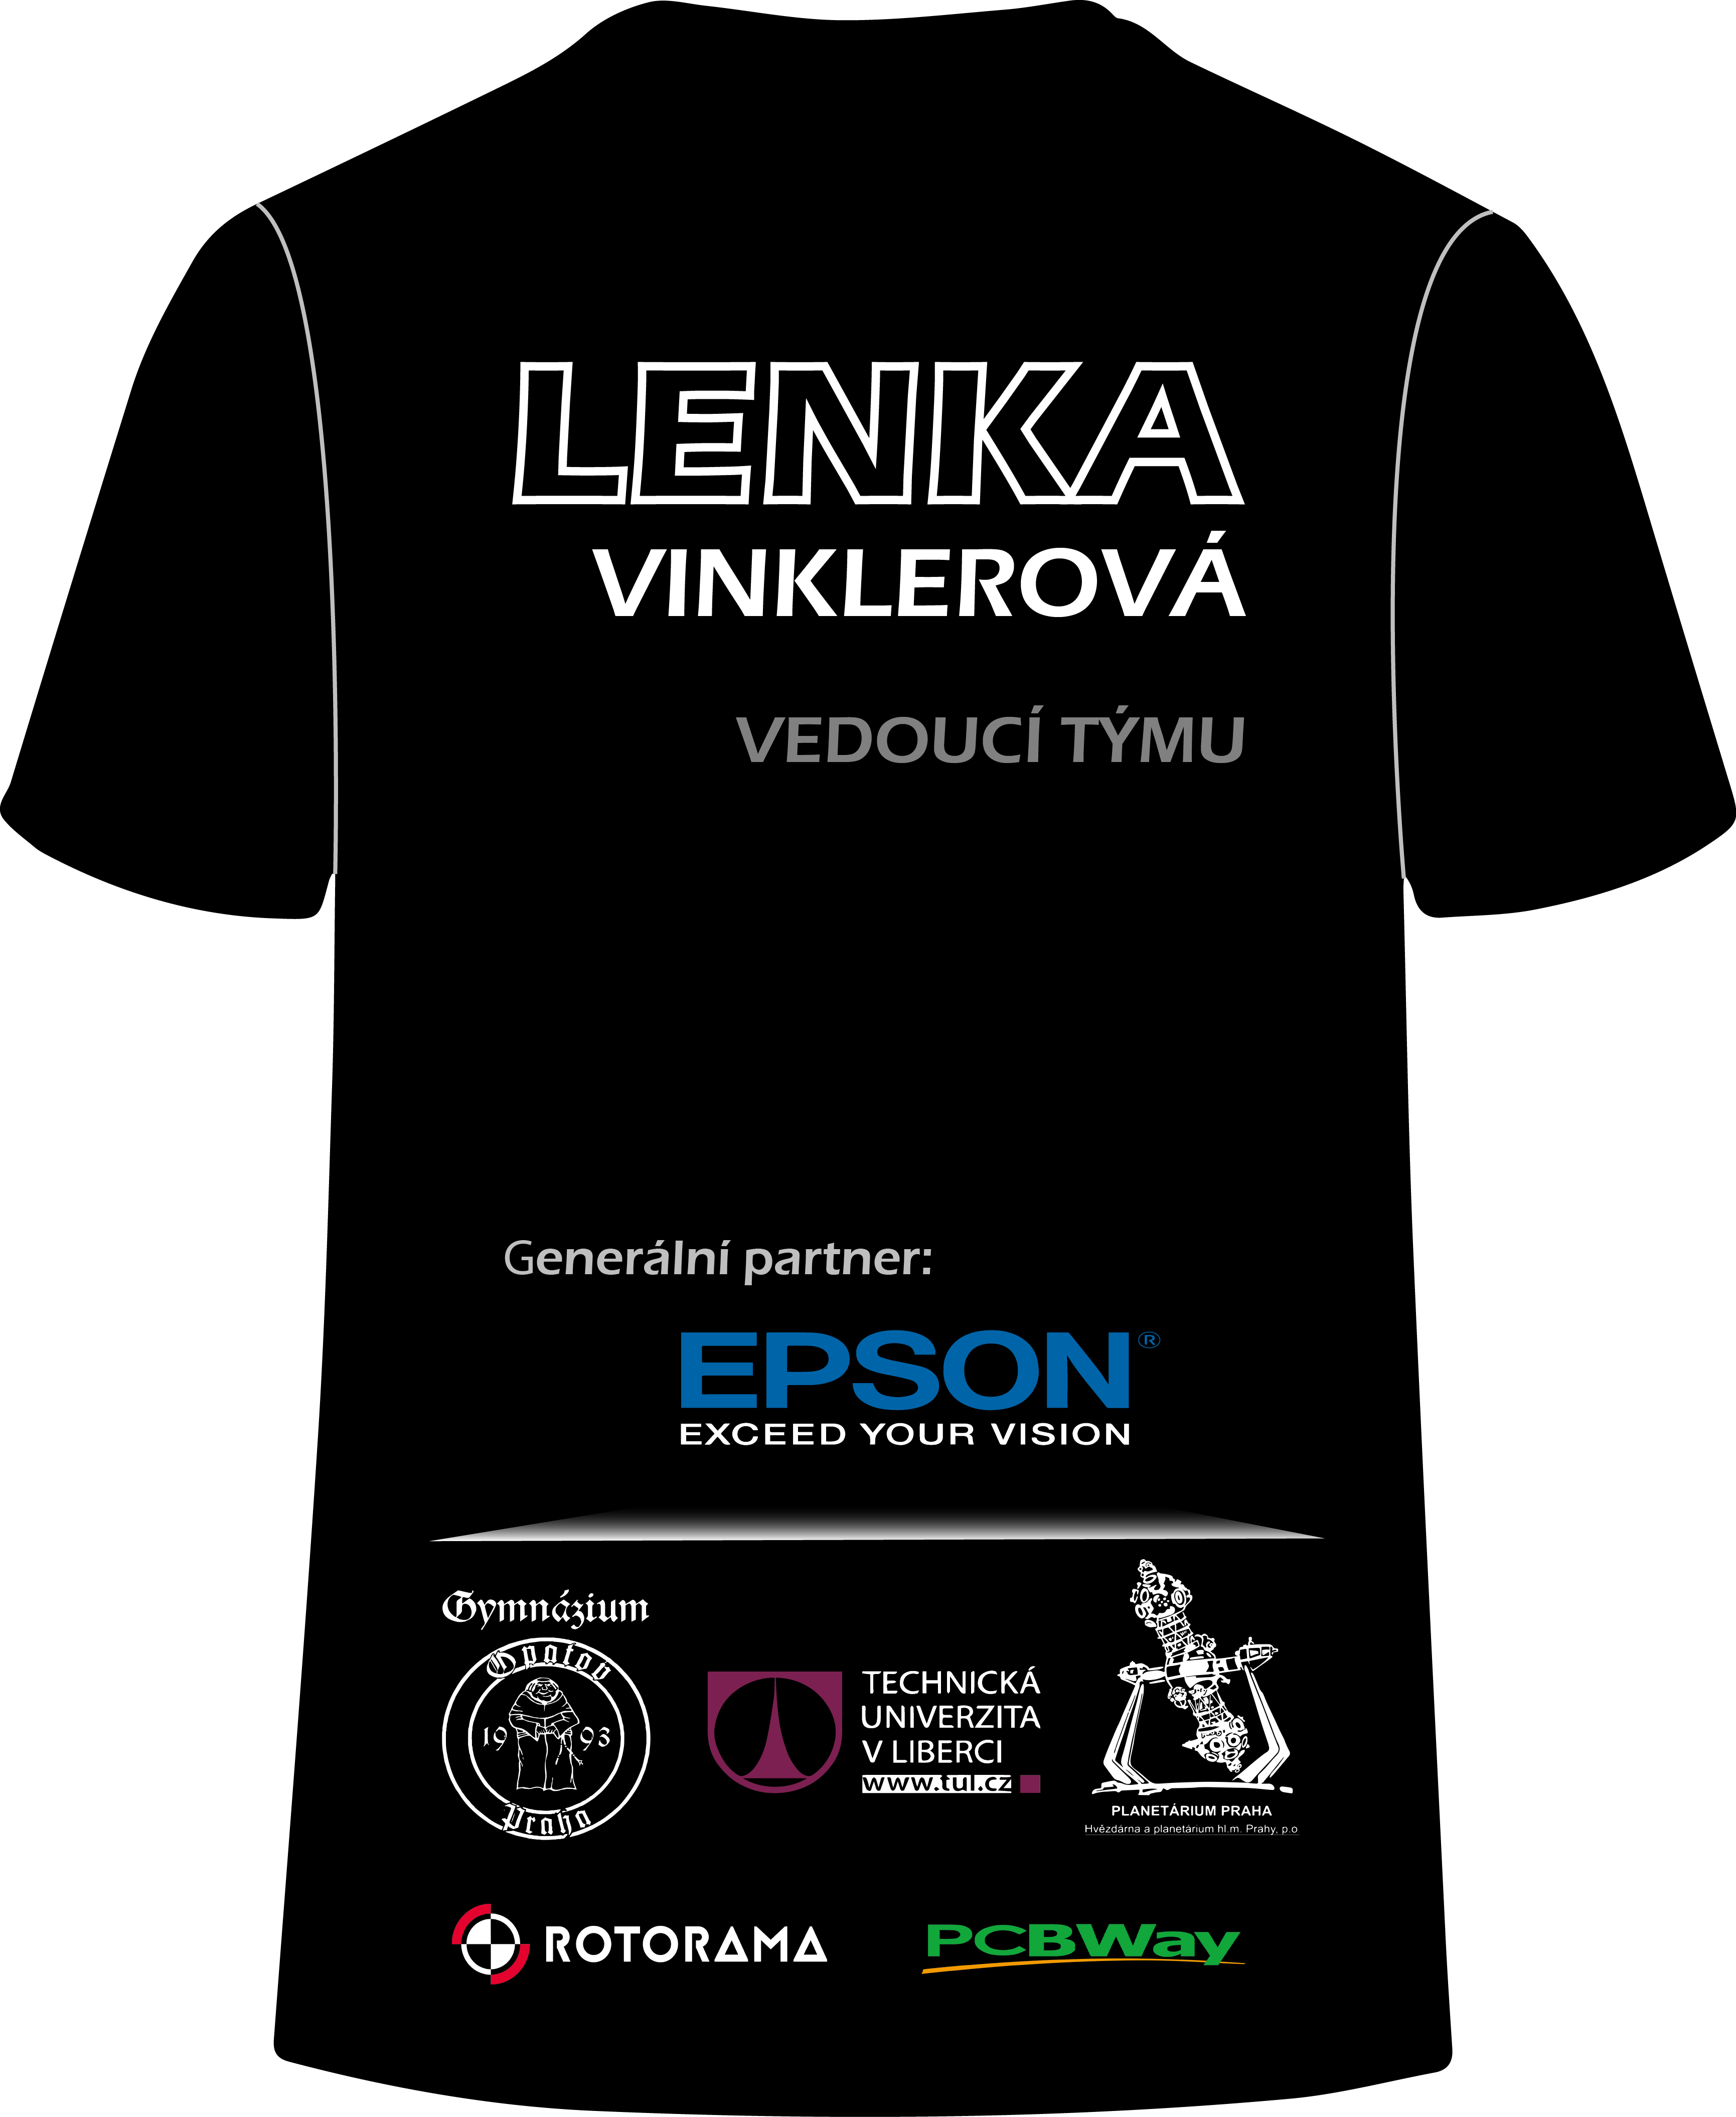
\includegraphics[width=500pt]{Triko_zada.png}
\end{figure}
\subsection{Konzultanti}
\paragraph{} Za konzultace patří speciální díky naší paní profesorce Lence Vinklerové, dále odborníkovi na telekomunikaci Zdeňku Mackovi a členovi týmu loňských a předloňských vítězů národního kola soutěže CanSat Janu Horákovi. Za pomoc při sjednávání kontaktů děkujeme panu Luboru Basíkovi. Nejen po nich jsme pojmenovali a plánujeme pojmenovat testovací i soutěžní lety.
\section{Publicita}
\paragraph{} Dne 4.dubna o nás vyšel článek ve školních novinách Gymnázia Opatov. Dále jsme navázali kontakt se Sekcí proměnných hvězd České astronomické společnosti, kdy jsme se s jejími členy 10. března spojili telemostem. Náš člen Patrik Novotný, účastník semináře ČAS, poreferoval o našem projektu, a poté jsme si vzájemně vyměnili zdravice a informovali o úspěších a neúspěších.
\paragraph{} Pro svá informační videa a videa z testů používáme \href{https://www.youtube.com/channel/UCbrLBa4NokHmF9CiW5-RHXA}{youtube kanál}, jenž jsme použili i pro streamování. Celý náš kód - programové vybavení CanSatu, modely, tato zpráva i mnoho dalšího je  dostupno na našem \href{https://github.com/suchanekj/CanSatGOSA}{GitHubu}. Ke komunikaci s podporovateli používáme ještě naši \href{https://www.facebook.com/GOSA-Gymn\%C3\%A1zium-Opatov-Space-Agency-1657994580942593/?ref=page_internal}{facebookovou stránku}, která je méně vážná než naše webové stránky, a slouží jako deník, včetně všech strastí i radostí.
\paragraph{} Společnost Epson nám zajistila spolupráci se známou PR agenturou \href{http://bisonrose.cz}{Bison \& Rose}. V současnosti s nimi domlouváme tiskovou zprávu, cituji:
\paragraph{} Tiskovou zprávu informující o tom, že budete bojovat ve finále – představujeme si ji v tomto duchu:
\paragraph{} Začátek by byl krátký popis samotné soutěže - o co jde. Dále by následovalo seznámení s Vaším projektem budeme čerpat zde: https://gosa.cz/Projects/CanSat/Backstory/ , prosíme také o nachystání Vaší citace – ideálně proč jste se rozhodl do projektu zapojit, co vám to přineslo atp... Následně bychom rádi zařadili citaci Katky Vymazalové za Epson – v duchu toho, že jsou rádi že se mohli finančně podílet na podpoře, tak skvělého projektu.
Chtěli bychom cílit na média:\\
\begin{itemize}
    \item Specializované weby: Sciencemag.cz, Czechspaceportal.cz, pocitacveskole.cz
    \item It weby: jako chip.cz, feedit.cz…
    \item Zkusili bychom oslovit i deníky – Pražský deník, Metro, Aktualně, e15.
    \item A také bychom chtěli zkusit nabídnout článek do časopisu ABC a oslovit TV ČT Déčko a jejich stránky.
    \item Zkusili bychom také oslovit zpravodajství českého rozhlasu.
\end{itemize}
\section{Doslov členů}
\begin{itemize}
\item Patrik Novotný: Pro mě osobně je CanSat náš společný příspěvek všem zájemcům o danou věc. Každý jsme do projektu vložili všechny své dosavadní znalosti a schopnosti, využili jsme své vědění naplno. Obvzlášť bych vyzdvihl obecnost našeho CanSatu, při změně programu je možno CanSat ovládat v reálném čase nebo s ním dokonce startovat jako s dronem. Vytvořili jsme velmi komplexní stroj schopný plnit celou řadu úkolů. Díky modulárnosti je možné měnit i čidla, pak by se náš CanSat dal využít i jako meteostanice nebo důlní sonda.
\item Jakub Suchánek: Už jsem se účastnil několika elektronických projektů, ale žádný nebyl veden takovým způsobem jako CanSat. Vždy šlo jen o to, abychom jakýmkoliv způsoben udělali robota, který dokáže splnit přesně zadaný cíl. Nikdy nikoho nezajímalo, zda jsme schopni nadchnout potenciální sponzory, či jak náš výtvor funguje. Vždy bylo jen kritérium, zda splnil úkol lépe než jiný robot, či ne. U CanSatu je to jinak. Domlouvání sponzorů byla úplně nová zkušenost, stejně jako psaní výstupních prací. Velmi tuto komplexnější formu soutěže oceňuji.
\item Lukáš Vőlfl: Projekt CanSat nám umožnil pracovat na něčem, k čemu bychom se nikdy sami neodhodlali. Ačkoliv jsme letos museli projít maturitním ročníkem, jsem přesvědčen, že každý člen do našeho společného projektu dával své maximum. Jako milovníka FPV závodních dronů mě samozřejmě potěšilo, když jsme se v září sešli a domluvili se na konstrukci podobné právě dronu. Bylo zajímavé sledovat vývoj celé konstrukce. Postupně se z našich představ stával opravdový funkční stroj se zvyšujícím se potenciálem uspět.  Nyní se řídí podle námi vytvořených algoritmů a je schopen autonomně přistát na „kterémkoliv“ místě. Na našem CanSatu se mi zdá však nejlepší, že je osazen moderními technologiemi, z nichž většina byla plně vyvinuta až v posledních pěti letech. Troufám si říct, že před třemi lety bychom vůbec nebyli schopni postavit stroj podobného konceptu. 
\item Jan Janoušek: GOSA a Cansat pro mě, jako letošního maturanta, znamenají možnost nechat po sobě něco hmatatelného po odchodu ze školy. I když nemám takové technické znalosti jako zbytek týmu, myslím si, že jsem schopen jim velmi pomoci jednoduchým pohledem na svět, nezatížený tím, zda daná věc ve skutečnosti opravdu jde zkonstruovat, nebo ne. Mojí hlavní činností bylo zajišťovat chod týmu, vozit členy na testování a starat se o naše kanály na sociálních médiích.
\item Jakub Zeman: Tato soutěž pro mě neznamená jen samotnou stavbu CanSatu, ale beru ji jako výzvu a příležitost dokázat, že umíme něco navíc, a taky ukázat, co dokážeme všichni dohromady. Každý z nás pracuje na částech, které jsou mu nejbližší, a právě v tom tkví síla našeho týmu. Nepochybně jsme také získali mnoho nových znalostí a zkušeností a to nejen v oblasti techniky.
Osobně mi dělá velkou radost, když porovnám své schopnosti před půl rokem a nyní a vidím pokrok a osobní rozvoj.
\item Martin Vítek: Když mi na začátku září byla představena soutěž CanSat, bral jsem ji jako zábavnou možnost si pohrát s elektronikou. Časem jsem však zjistil, jaké možnosti tato soutěž skrývá. Je to možnost vyzkoušet si práci na projektu relativně větších rozměrů a se vším všudy i práci v týmu, tak jak jsem ji doposud nepoznal. Mimo to jsem také rozšířil své obzory nejen v elektronice a konstrukci, ale i v oblasti publicistiky a práva. Zároveň jsem si zkusil programovat komplexnější programy, které jsou užitečné a prakticky využitelné. CanSat pro mě byl a doufám, že ještě bude, velmi dobrou zkušeností.
\end{itemize}
\begin{figure}[!h]
\centering
\caption{Společná fotografie,zdroj: GOSA}
\includegraphics[width=400pt]{Spolfoto.jpg}
\end{figure}
\section{Závěr}
\paragraph{} K projektu by šlo napsat ještě mnoho, ale je potřeba znát míru informací, kterou chce člověk předat. Nemělo by to být ani málo ani moc. Rádi odpovíme na vaše případné další dotazy. Tato zpráva není určena jen hodnotitelům soutěže, ale i všem našim chlebodárcům, jakož i komukoliv, koho projekt a jeho pozadí zajímá. Ostatně zdrojový kód této zprávy je dostupný na našem GitHubu. Zprávu jsme se snažili vypracovat dle vědeckých standardů, proto je také vypracována v programu \LaTeX. Nezvolili jsme si lehkou cestu. Prozatím dle našich testů však všechny naše systémy fungují a u těch kritických jsme připraveni i na případný problém. Finální ortel vynese národní finále. Víru v to, že se náš projekt ukáže v nejlepším světle, vyjadřuje citát Henryho Forda: \say{Schopnost nadšení nese tvé naděje ke hvězdám.}
\section{Zdroje-Inspirace}
Z následujících webových stránek jsme čerpali informace či se jimi inspirovali pro dané řešení:
\begin{itemize}
\item\href{http://www.vk2zay.net/article/265}{Alan's Lab - Photodiode Gamma Ray Detector}
\item\href{https://earthobservatory.nasa.gov/Features/UVB/}{NASA EO/Jeannie Allen - 	
Ultraviolet Radiation: How it Affects Life on Earth}
\end{itemize}
\listoffigures
\end{document}